% USC Dissertation/Thesis LaTeX Template
% Edited by Ruda Zhang, 2020-10-08.
% -----------------------------------------------------------------------------
%	PACKAGES AND DOCUMENT CONFIGURATION
%-----------------------------------------------------------------------------

% Use `report` class with `USCthesis` package (style file) by Brian P. Gerkey
% Font size should be 11 or 12 points for regular paragraph text.
\documentclass[letterpaper,12pt]{report}
% [options] can be any of these default/alternative flag:
%   dissertation/thesis, final/proposal, copyright/nocopyright,
%   fussy/sloppy, flushbottom/raggedbottom, clref/opref.
\usepackage[proposal]{USCthesis}

% Packages required by `USCthesis.sty`.
\usepackage{hyperref}
\usepackage{setspace}
\usepackage{tabularx}

% Line spacing and margins in compliance with USC graduate school guidelines.
\usepackage[margin=1in,footskip=.5in]{geometry}
\doublespacing

% Optional packages: mathematical fonts and symbols
% You may comment this section out if you don't need them.
\usepackage{mathptmx} % set font to Times Roman
\usepackage[OT1]{fontenc} % font encoding for xelatex
\usepackage{mathtools}
\usepackage{amsmath}
\usepackage{amssymb}

% Optional packages: graphics
\usepackage{graphicx}
% You can use the "demo" option while editing to avoid compiling figures.
% \usepackage[demo]{graphicx}
% You can add absolute paths as well.
\graphicspath{{./}{../}{figures/}{../figures/}}

% Optional packages: bibliography with BibLaTeX.
% Comment this section out if you prefer BibTeX.
\usepackage[
    style=nature,
    sorting=none,
    isbn=false,
    url=false,
    doi=true,
    eprint=false,
    date=year,
    maxnames=6,
    minnames=6
]{biblatex}
\AtEveryBibitem{\clearfield{eventtitle}} 
\AtEveryCitekey{\clearfield{eventtitle}}
\AtEveryBibitem{\clearfield{pagetotal}} 
\AtEveryCitekey{\clearfield{pagetotal}}
\addbibresource{references.bib}

% Filler text for formatting. Comment these lines out for real writing.
\usepackage[english]{babel}
\usepackage{blindtext}


\begin{document}

%-----------------------------------------------------------------------------
%	TITLE PAGE
%-----------------------------------------------------------------------------

% Volume name could be added as option, e.g. `[Volume I]`.
\title{\textbf{\Large{Writing a thesis at USC}}}

\author{Tommy T. Trojan}

% Committee list is only shown in `proposal` layout.
\committee{A.~Adams & (Chair)\\*
           B.~Bell\\*
           C.~Clausius\\*
           D.~Dirichlet\\*
           E.~Emory & (Outside Member)}

% Submission information is only shown in `final` layout.
\majorfield{Civil Engineering}
\submitdate{December 2020}  % Must be one of the three dates allowed in the guideline

% Make sure everything, specially your title page, exactly follows the guideline:
% https://graduateschool.usc.edu/wp-content/uploads/2020/11/Manuscript_Formatting_and_Documentation_Styles.pdf

%-----------------------------------------------------------------------------
%	PREFACE
%-----------------------------------------------------------------------------

% The preface environment prints the title page.
\begin{preface}

  % Dedication Page, which is truly unnecessary.
  \prefacesection[Dedication]{}
  \input{dedication}

  % Acknowledgement Page, which is also unnecessary for proposals.
  \prefacesection{Acknowledgements}
  \input{acknowledgements}

  \tableofcontents
  \listoftables   % Comment this out if you don't have tables
  \listoffigures

  % Abstract Page
  \prefacesection{Abstract}
  
In today's information-rich landscape, there has been a rapid rise in content available through web-based platforms reliant on diverse modalities. Multimodal content can manifest in varied forms like online news articles, movies, advertisements, and digital short videos. Our ability to comprehend the underlying narratives in these sources depends on the integration of various modalities, including audio, visual, and language. Further proliferation of multimodal content across diverse platforms necessitates a large-scale understanding of its impact on individuals and society as a whole. 
\par
In this work, we consider the problem of multimodal content understanding at diverse scales to obtain a holistic view of the input sources. Further, our approach to content understanding is reliant on contextual information processing from multimodal input sources. We process diverse forms of contextual information through various modalities and integrate the same using context-guided attention mechanisms. We show that the inclusion of context information improves multi-scale content understanding across a variety of input sources like movies, advertisements, TV shows, and natural scene images. We further conclude by providing directions for future research where we would like to explore information theoretic approaches for extracting optimal representations from context-guided attention mechanisms.







\end{preface}

%-----------------------------------------------------------------------------
%	CONTENT STRUCTURE
%-----------------------------------------------------------------------------

% Better to separate LaTeX structure and content
\chapter{Introduction}
\label{cha:introduction}
This chapter provides the necessary background material and details the organization of my proposed work.

\section{Multi-modality}
\subsection{Modalities - Definition and Introduction}
\textit{Modality refers to the way something happens around us or is perceived by humans} \cite{Baltruaitis2017MultimodalML}. The world around us is composed of multiple sensory modalities, as listed below, with enabled capabilities:
\begin{itemize}
    \item \textbf{Visual:} Watching objects and events in the current visual scene
    \item \textbf{Language:} Verbal interactions with other humans 
    \item \textbf{Audio:} Speaking and hearing environmental sounds 
    \item \textbf{Touch:} Feeling texture of objects 
    \item \textbf{Smell:} Distinguishing between pleasant and unpleasant odors.
\end{itemize}
For humans, the information from multiple sensory sources is processed by distinct regions of the brain for different perceptual tasks \cite{Alain2001WhatA,BornkesselSchlesewsky2015NeurobiologicalRO,Wallace2002HistochemicalIO}. While the visual input processing is handled by the occipital lobe in the brain, the auditory and language inputs are processed by specific regions of the temporal lobe. The sub-division of the human neural processing system into regions that can process a wide variety of modalities indicates the heterogeneity among different sources along with underlying commonalities, as shown in Fig \ref{cerebral_cortex_modalities}.

\begin{figure}
    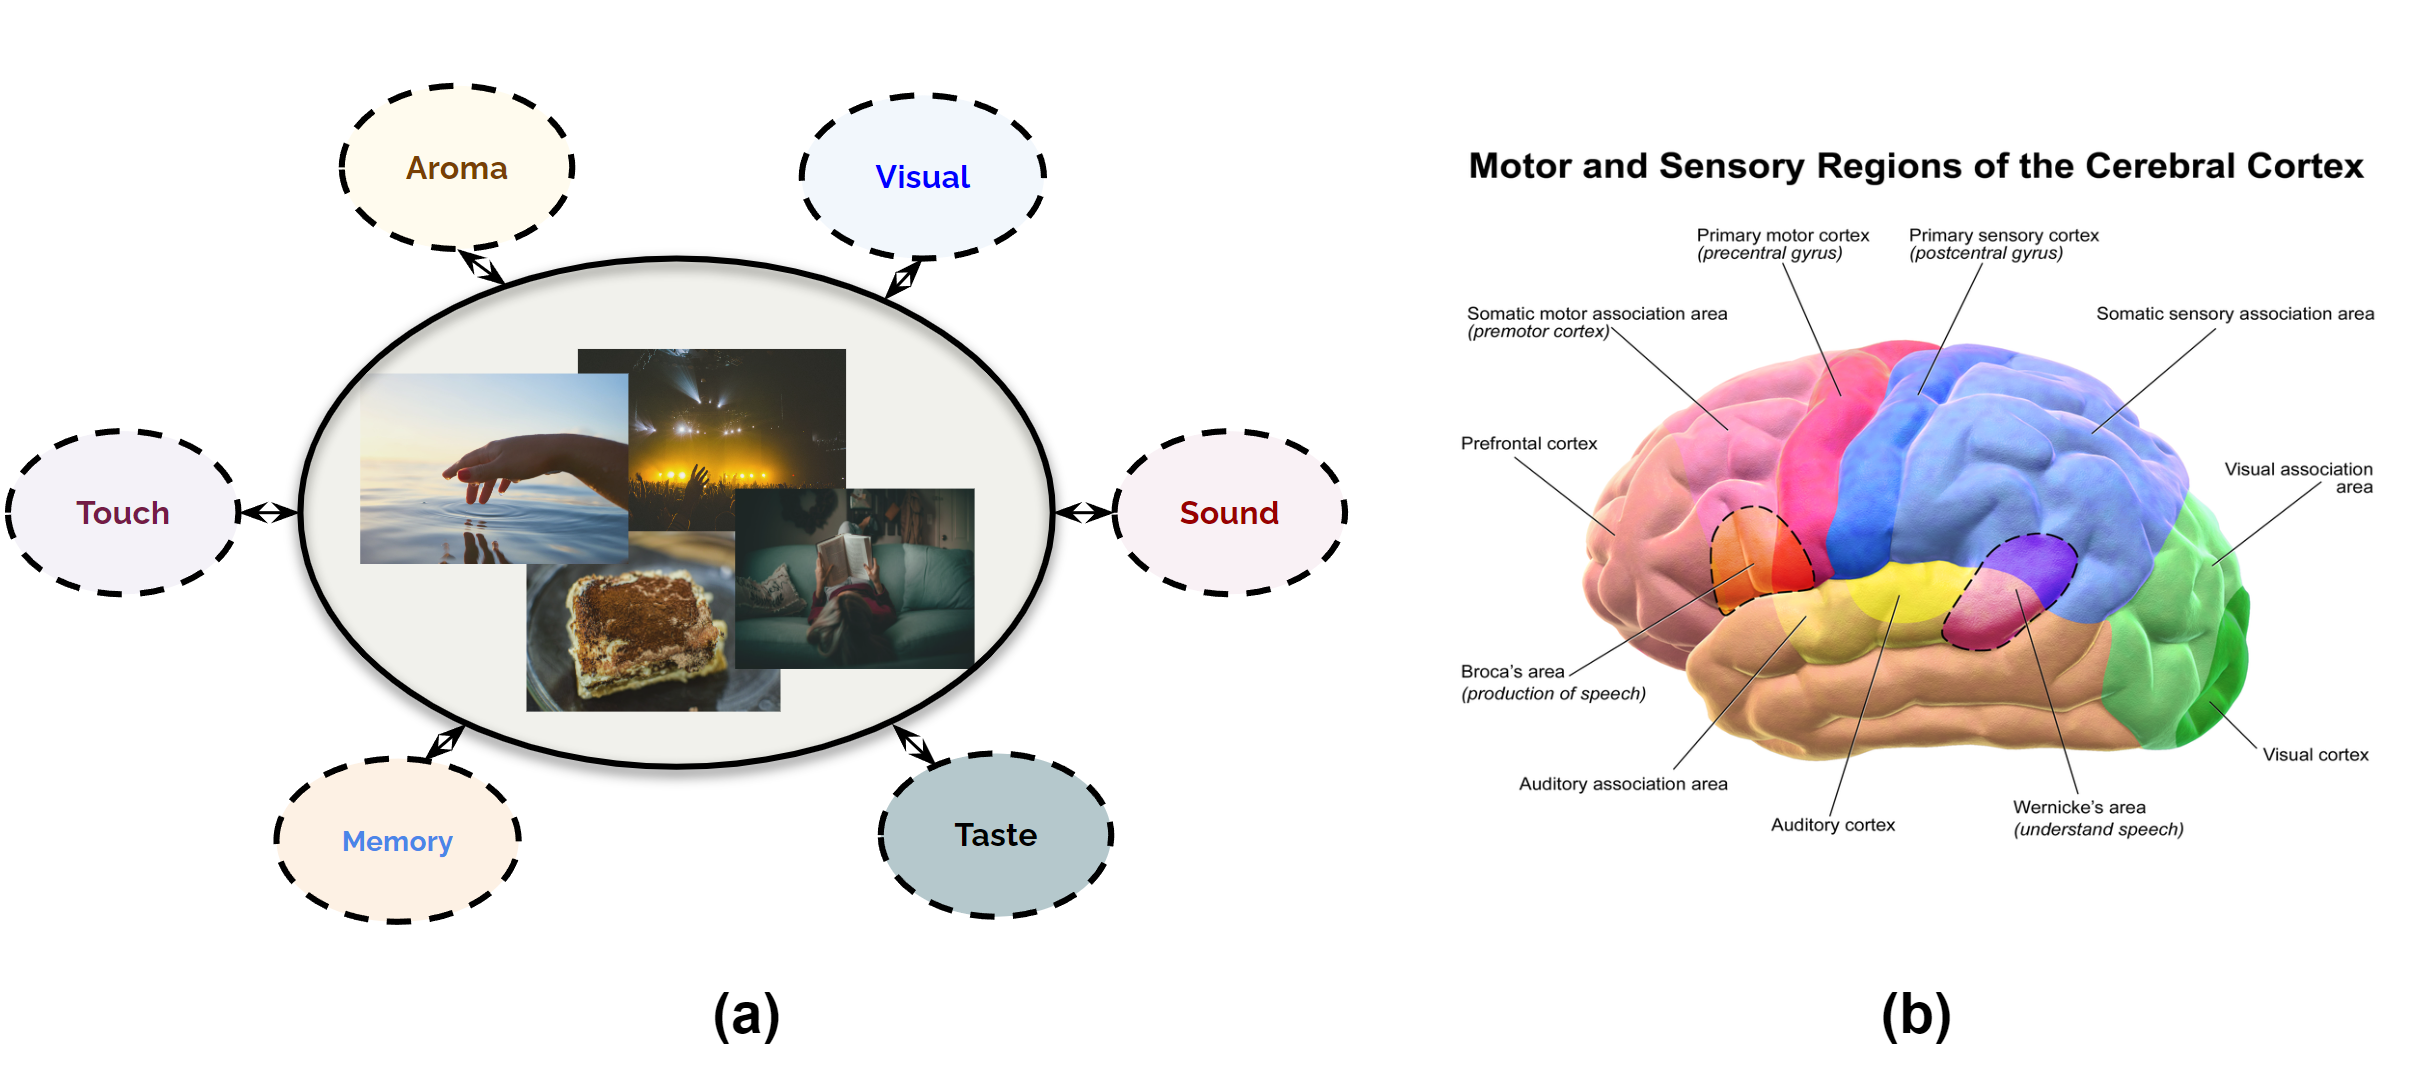
\includegraphics[width=\textwidth]{figures/cererbral_cortex_multiple_modalities.png}
    \caption{ (a)  Sensory modalities associated with real-world human perception  (b)  Specialized regions in brain where sensory information comes together and processed by different cortices}
    \label{cerebral_cortex_modalities}
\end{figure}

In artificial intelligence, a given task is considered multi-modal if multiple sensory modalities are needed to solve the same. The goal of artificial intelligence is to develop autonomous agents that can learn from diverse input modalities to solve complex reasoning tasks. As mentioned by Liang et al. \cite{Liang2022FoundationsAR}, the key properties associated with learning from multimodal data are listed as follows:
\begin{itemize}
    \item \textbf{Heterogeneity:} Heterogeneous nature of different modalities due to diversity in qualities, structures, and representations
    \item \textbf{Connectedness:} Shared/common information between different modalities due to inter-related nature.
    \item \textbf{Interaction:} Existence of optimal interactions/fusions between different modalities, suitable for particular task.
\end{itemize}
Based on the above properties associated with multiple modalities, the major challenges in multimodal learning \cite{Liang2022FoundationsAR} can be summarized below:

\begin{itemize}
    \item \textbf{Representation:} Learning representations through fusion mechanisms that capture the heterogeneity of the modalities along with the shared information. For example, language is considered symbolic due to its word-based composition, whereas audio and visual modalities are represented through signals.
    \item \textbf{Alignment:} Identifying relationships between (sub) elements of different modalities. This requires similarity computation between different modalities along with the handling of long-term dependencies.
    \item \textbf{Reasoning:} Combining knowledge from multiple sources (including external, i.e. knowledge graphs) in a multi-step inference process by exploiting the task structure.
    \item \textbf{Generation:} Translating between different modalities and summarization of multimodal data by preserving the salient content.
    \item \textbf{Transference:} Transferring cross-modal knowledge from secondary modalities to the primary modality in the presence of noise or limited data.
\end{itemize}

% In this work, we deal with the alignment, reasoning, and transference challenges associated with multi-modal learning.
    
\subsection{Rise of multi-modal content}

With the rapid rise in heterogeneous internet networks across the globe, vast amounts of web-based content have been generated at different scales, variety, and velocity \cite{Gao2020ASO}. Web-based sources convey information to the viewers through a combination of multiple modalities. For example, an online news article about a major sports event contains text descriptions with accompanying images. Further, the movies or TV shows hosted through online streaming platforms portray narratives through the combination of video and audio signals (music, speech, ambient sounds). 
The demand for media content, especially movies, TV shows, and advertisements, is expected to rise over the next three years, with the projected market value to reach 2.9 trillion US dollars, as shown in Fig \ref{media industry demand}.
\begin{figure}[h!]
    \centering 
     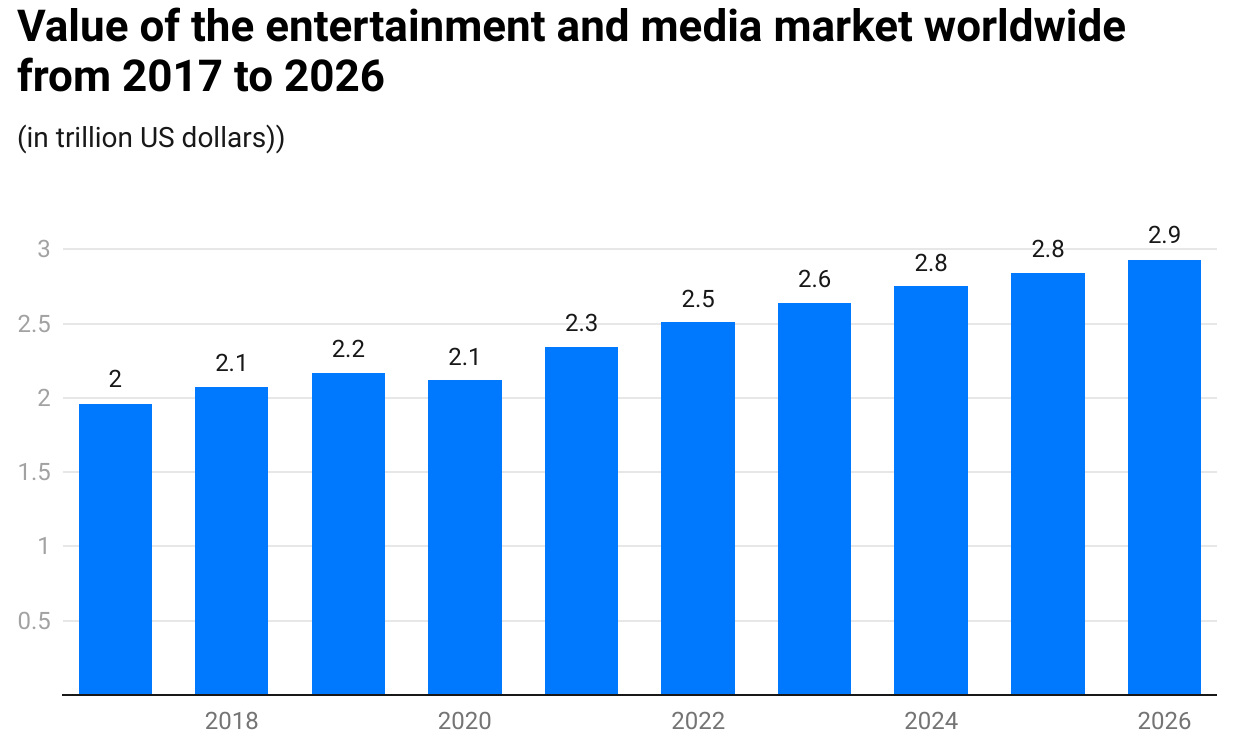
\includegraphics[width=0.6\linewidth]{figures/media_industry_demand.png}
     \caption[Media value]{Expected value of entertainment market industry from 2017 to 2026 \footnotemark} 
     \label{media industry demand}
\end{figure}
\footnotetext{\url{https://www.enterpriseappstoday.com/stats/media-and-entertainment-industry-statistics.html}}
The growing demand for multi-modal media content has led to various descriptive tasks such as captioning \cite{Abdar2023ARO}, video summarization \cite{Apostolidis2021VideoSU}, and question-answering \cite{defaria2023visual}, aimed at enhancing user experience. In the following sections we will introduce the concept of context and how multiple modalities provide contextual information.

\section{What is context ?}
In computer vision, context \cite{contextvision} refers to any relevant information encompassing the attributes of the object and event considered, along with other entities (objects and events) in the given scene, both visual and non-visual. Contextual information enables a wide variety of tasks, including object recognition, human affect perception, and salient event detection in videos, by providing additional cues needed for accurate inference. For example, the visual scene in a given image provides the necessary contextual information to detect commonly co-occurring objects along with any atypical placements. In terms of object placements, utensils are more likely to be found in the kitchen as compared to bedrooms or stadiums. An example of context providing the required information to improve object recognition under challenging conditions (poor lighting, image blurring, ) is shown in Fig \ref{object recognition}. The blurred object (marked by a red circle), when viewed in isolation, is not recognizable. However, when the object is placed in the context of the entire visual scene i.e. office, we can see that it is likely to be a keyboard.
\begin{figure}[h!]
    \centering 
     
\includegraphics[width=0.6\linewidth]{figures/blurred_object.png}
     \caption{ \textbf{LEFT:} A blurred object (marked in red circle), when viewed in isolation, is not recognizable. \textbf{RIGHT:} Contextual information in the form of the visual scene helps in recognition. Image source: \cite{Marques2010ContextMI}}
     \label{object recognition}
\end{figure}

Context also refers to the situation surrounding our responses and actions \cite{baez2018does}. An example of situational context can be seen in Fig \ref{context situation}. When the face is only considered, it conveys pain. However, by taking the entire situation into context involving the celebration, it can be inferred that the person is happy based on bodily expressions and the event (sports match). 

\begin{figure}[h!]
    \centering 
    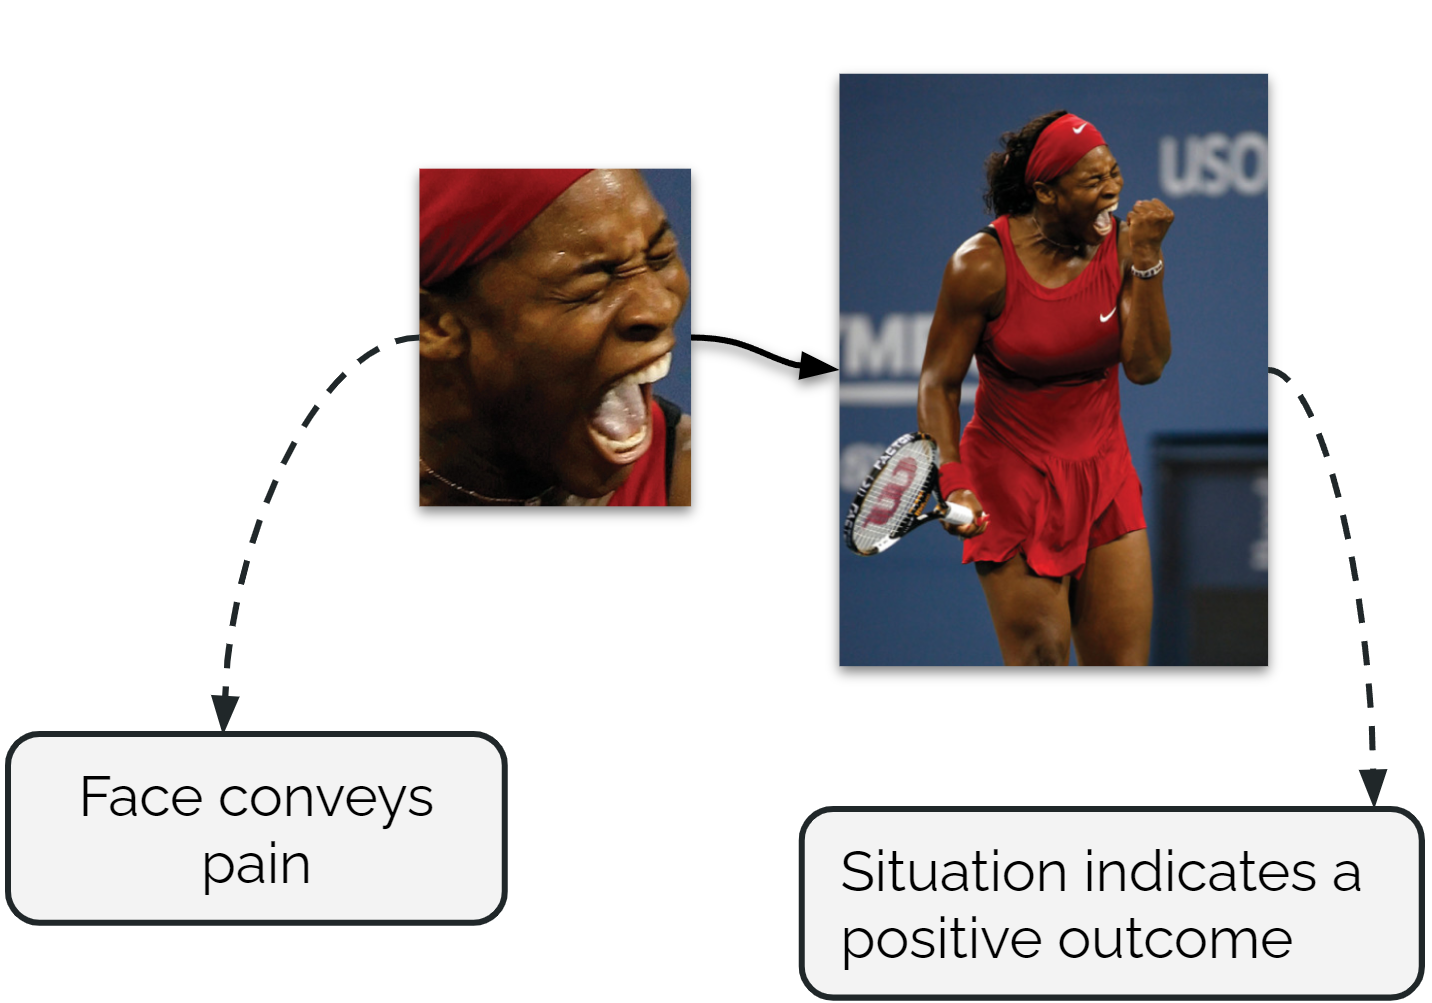
\includegraphics[width=0.6\linewidth]{figures/context_situation.png}
    \caption{Example of the situation as context information. Image source: \cite{barrettcontext} }
    \label{context situation}
\end{figure}


The broad organization of different context sources, along with associated levels is shown in Fig \ref{Context_type}.
\begin{figure}[t]
  \centering
  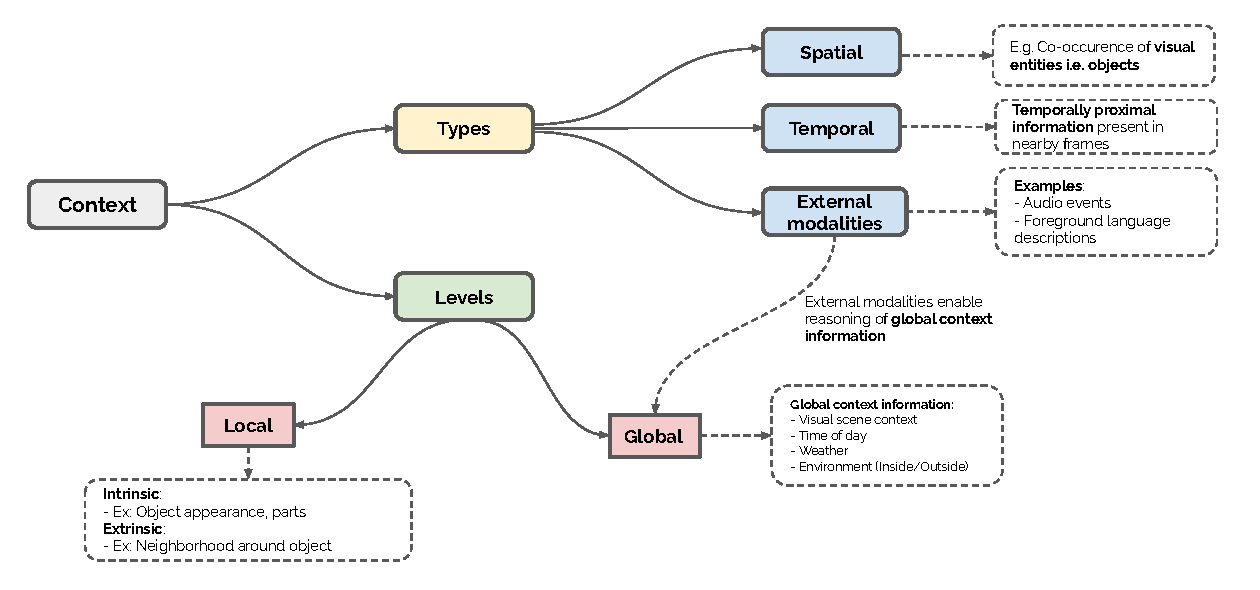
\includegraphics[width=\linewidth]{figures/Context_type.pdf}
  \caption{Variations in types and levels of context. Outline of context levels and types inspired from Fig 5 in \cite{contextvision}.}
  \label{Context_type}
\end{figure}
Context can be broadly divided into three types as follows:

\subsection{Spatial context}
Spatial context refers can be defined as the \textit{possibility of finding objects located at certain positions in the scene w.r.t other proximal objects}. For example, a ship can be found floating at sea rather than on a highway.
Spatial context can be further subdivided into the following major classes:
\begin{itemize}
    \item  \textbf{Spatial co-occurrence}: Spatial co-occurrence can be leveraged through co-occurrences of object labels in the same visual scene. Rabinovich et.al \cite{Rabinovich2007ObjectsIC} utilized co-occurrence statistics between labels in a CRF-based framework to refine object detections in a given visual scene. Further, Wang et al. \cite{Wang2007ShapeAA} expanded the idea of co-occurrence by providing a probability distribution of labels over different regions based on a given pixel location. Yang et.al \cite{Faceness-Net} explored fine-grained relative spatial information between facial parts i.e., placement of nose, mouth for face detection. 
    \item  \textbf{Direction and toplogical relations}: 2-D spatial relations between entities can be described through direction and topological-based relations \cite{Marques2010ContextMI}. Directional relations deal with the proximity of one object with other objects in terms of other entities based on relative terms like \textit{"near"}, \textit{"above"}, \textit{"below"}. Whereas topological relations are concerned with the neighborhood of the objects in terms of overlap/containment with distinct regions i.e. exterior, boundary and interior.
    \item  \textbf{Semantic driven spatial context}: Semantic context restricts the space of possible spatial contextual relations in a given scene to a set of valid ones. The usage of semantic context between proximal objects enables correction of mislabeling in images \cite{Rabinovich2007ObjectsIC}, and accurate discovery of all possible valid relations between objects through scene graphs \cite{Chang2021ACS}. An example of a scene graph with entities and semantic relations obtained after message-passing operations \cite{Xu2017SceneGG} is shown in Fig \ref{scenegraph}.
    \begin{figure}[h!]
    \centering
        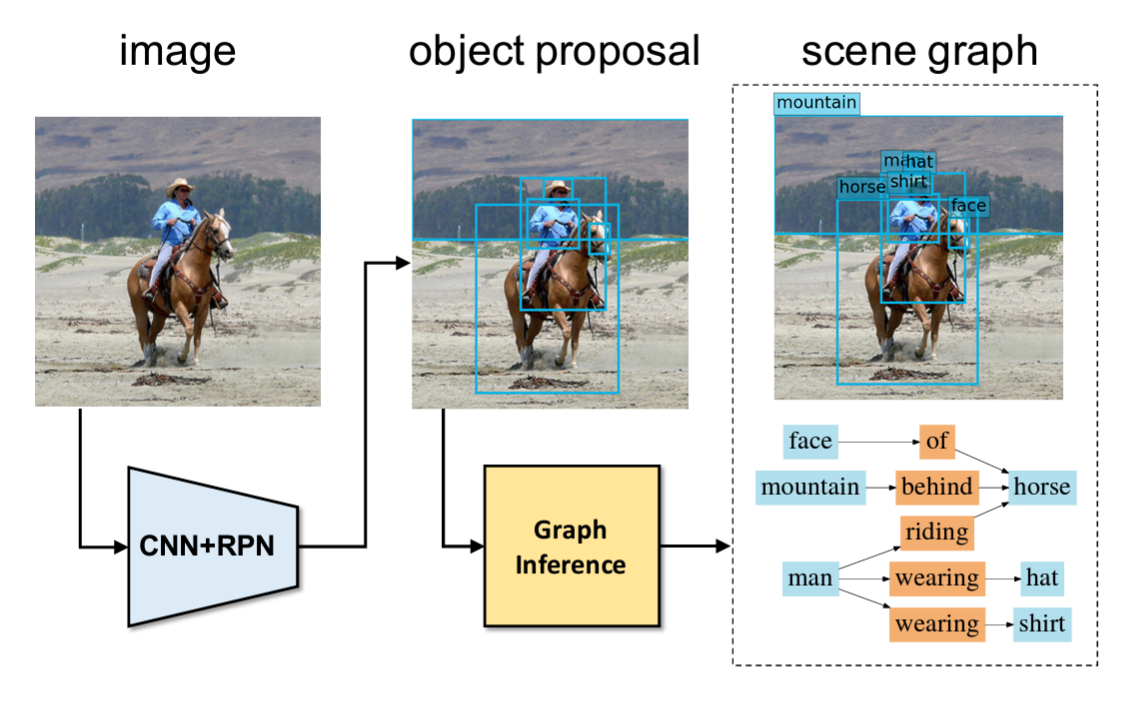
\includegraphics[width=0.5\linewidth]{figures/Scene_graph_outline.png}
        \caption{Sample scene graph obtained after iterative message passing (graph interface) over the region proposals (objects) }
        \label{scenegraph}
    \end{figure}
\end{itemize}

\subsection{Temporal context}
Temporal context refers to the \textit{information present in dynamic content, i.e. nearby or distant frames in videos}. The major subdivisions of temporal context are listed as follows:
\begin{itemize}
\item \textbf{Short-term temporal context:} Short-term temporal context relies on information present in nearby frames, which can be a short temporal window centered on the current frame or previous frame. The temporal context within a short window, (usually a few seconds) enables general video understanding tasks, including action recognition \cite{Carreira2017QuoVA}, pedestrian tracking \cite{Yan2019LearningCG}, human-object interaction \cite{Ji2021DetectingHR}. 
\item \textbf{Long-term temporal context:} Instead of limiting to nearby frames, long-term temporal context deals with temporal scale spanning from hours to months/years. General media-focused tasks based on movies \cite{Wu2021TowardsLV,Soldan2021MADAS} rely on long-form narratives (usually minutes to hours) for understanding character interactions, event dynamics, and broad semantics, including genre, etc. For tasks like species monitoring, temporal information over extended periods of time (months or years) is required for accurate identification \cite{Beery2019ContextRL}. 
\end{itemize}
In spite of clear divisions between short-term and long-term temporal contexts based on the duration of information, certain narrative-driven videos in media, i.e., advertisements, contain: 
\begin{itemize}
\item Rapid changes in short-term contextual information based on shots. 
\item Long-term contextual association between the shots based on an integrated narrative.
\end{itemize}
\subsection{External modalities}
Apart from visual-only information, modalities such as audio, language, and prior weather information also provide relevant contextual information for various reasoning tasks. For example, in the case of audio-visual tasks, the audio associated with an entity, i.e., dog barking, can help us estimate the proximity of the sound source and localize it in the given video \cite{Tian2018AudioVisualEL}. Further usage of audio modality as an additional contextual source for visual tasks has been explored in floorplan design \cite{purushwalkam2020audio} and audio-visual navigation for virtual agents \cite{chen2020soundspaces}. For various vision-language tasks like temporal grounding, natural language queries can be used as contextual inputs to isolate regions of interest in unconstrained videos \cite{Zhang2022TemporalSG}. Besides language and audio, additional contextual information available through thermal sensors \cite{Seymour2017AutomatedDA} is used to augment the visually captured data for improving wildlife detection in remote areas. In case of affect understanding problems, multi-turn dialogues (\textbf{language modality}) provide the necessary context information (i.e. topics and flow of information) along with facial expressions for emotion tracking of the speakers \cite{Zhao2022M3EDMM}.

\subsection{Local context}
Local context refers to the \textit{contextual information associated with objects itself (\textbf{intrinsic}) and surrounding local regions (\textbf{extrinsic}) such as color, shape, contrast, aspect ratio} \cite{contextvision}. Local context is closely related to spatial information in terms of the immediate neighborhood of the objects in the scene. Effective utilization of local context enables the detection of small objects in complex scenes with multiple entities. External modalities often provide local context for multi-modal reasoning, i.e., the conversation history (\textbf{language}) enables the autonomous agent associated with visual dialog \cite{Das2016VisualD} to provide the correct in-context answer.

\subsection{Global context}

Global context utilizes \textit{the overall configuration of the scene as a source of contextual information \cite{contextvision}}. The primary sources of global context information are as follows:
\textbf{(A) Visual scene:} The visual scene where the objects are present, i.e. living room, kitchen, train station etc. \\
\textbf{(B) Time of day:} The timing shown in the given image/video i.e. day, night, evening, or morning. \\
\textbf{ (C) Weather:} The ambient weather conditions associated with the given scene, i.e. sunny etc. \\
\textbf{ (D) Environment:} The environment associated with the given scene i.e., inside or outside.
\par 
Visual scene, along with the associated environment provides the prior context for finding certain objects. For example, there is a greater likelihood of finding utensils in the kitchen (\textbf{indoor visual scene}) as compared to train station (\textbf{outdoor visual scene}). Global context information (in the form of visual scenes) also influences the relative placement of different objects, like the proximity of a keyboard to the monitor in an office setup. Further, the accurate identification of different objects as part of the local contextual information in a given image/video can also help 
in recognizing the given visual scene \cite{Torralba2003ContextualPF} and its attributes (i.e., indoor/outdoor, time of day, etc.). For example, the presence of a microwave oven and dishwasher indicates that the visual scene is likely a kitchen. The global context information can also help in identifying atypical scenarios \cite{Choi2012ContextMA} involving objects i.e., a car located in the sky or a plane running on a highway, as shown in Fig \ref{outcontext}. 
\begin{figure}[h!]
    \centering
        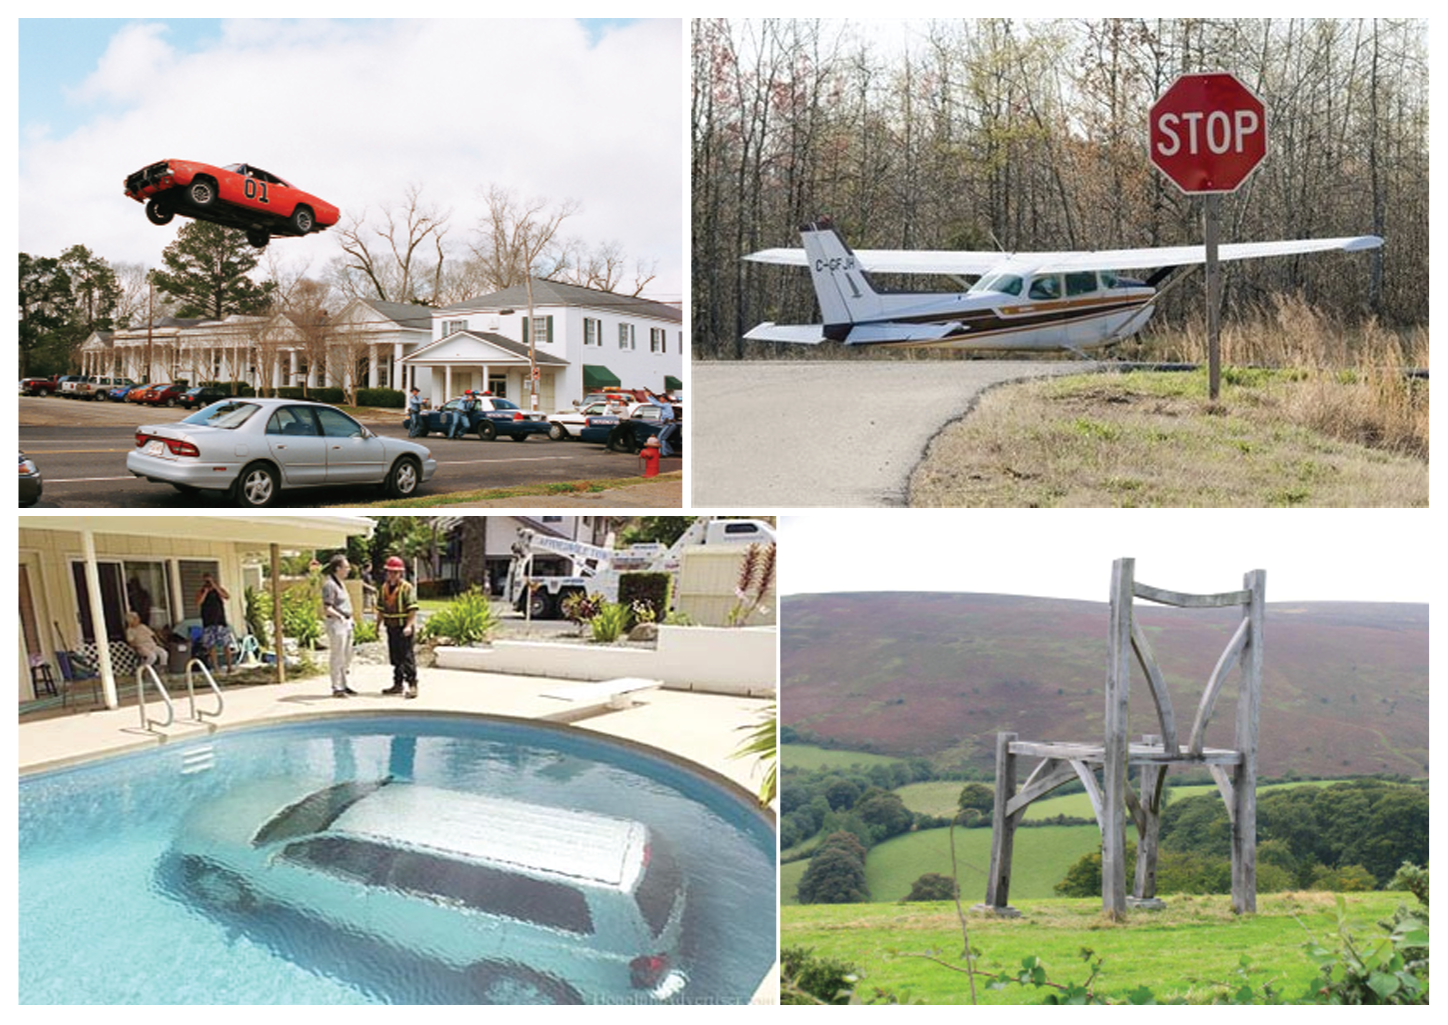
\includegraphics[width=0.5\linewidth]{figures/out_of_context_image.png}
        \caption{Sample images from \cite{Choi2012ContextMA} showing atypical scenarios involving violations of support, position, probability, size }
        \label{outcontext}
\end{figure}
    
\section{Context-driven multi-modal understanding}
\begin{figure}[h!]
    \centering
        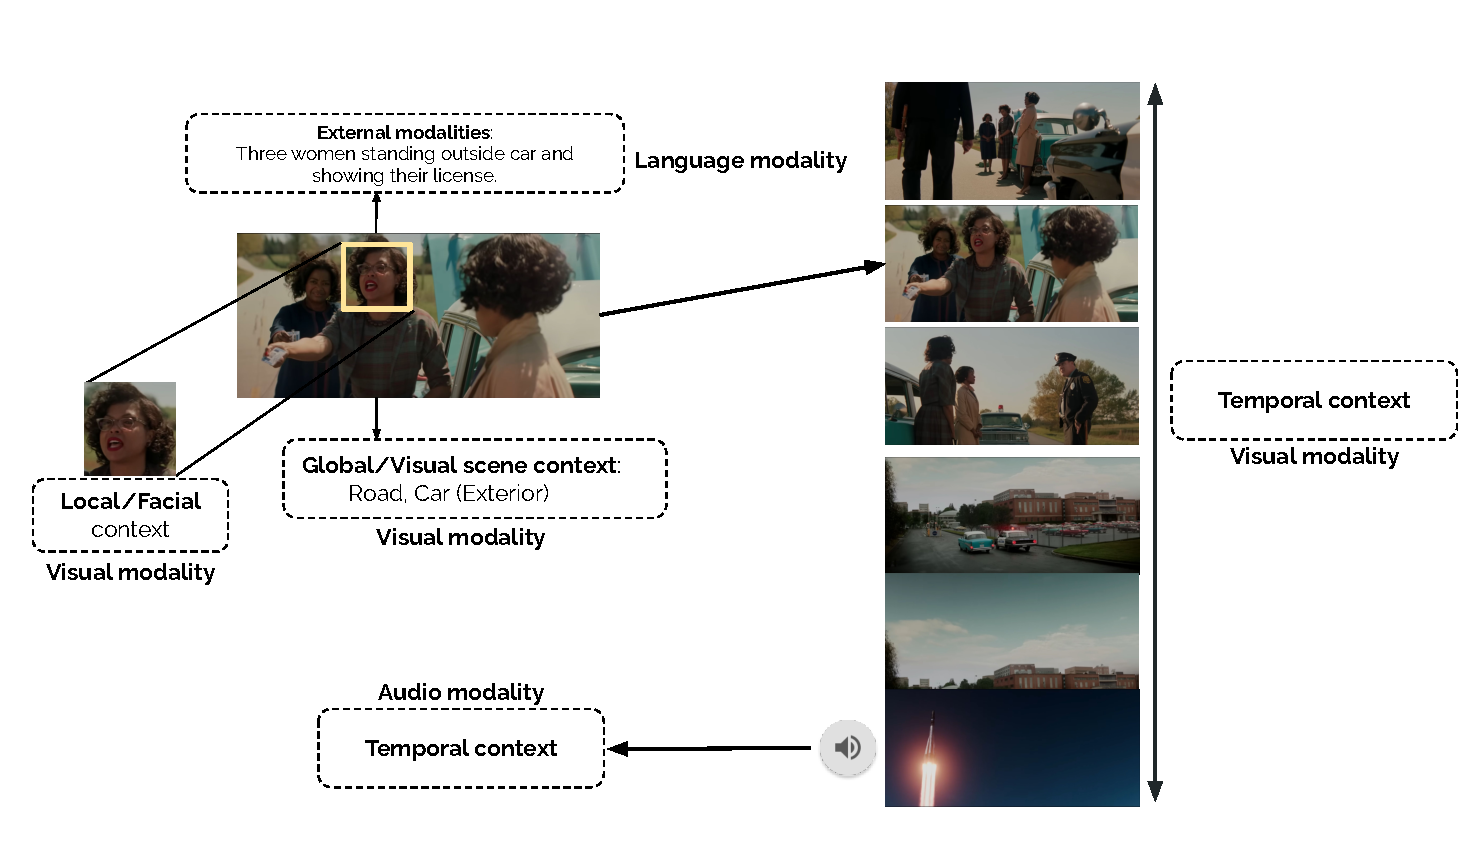
\includegraphics[width=0.9\linewidth]{figures/context_diagram.pdf}
        \caption{Outline diagram showing the presence of various contexts and associated modalities in a sample movie clip.} 
        \label{contextmultimodal}
\end{figure}
Multi-modal tasks require the processing of diverse contextual information followed by fusion for both macro and instance-level content understanding. In the case of multi-modal content, the contextual information is usually obtained through multiple input modalities. In \textbf{Fig \ref{contextmultimodal}} \footnote{Hidden Figures (2016): https://www.youtube.com/watch?v=W1VZ1-ZdQ7k\&ab\_channel=20thCenturyStudios}, we can see that the face crop of the person captures the \textbf{local/facial} context in the frame of interest. The \textbf{global} context is captured by visual scene i.e., \textbf{road, car (exterior)}. External modalities in the form of natural language descriptions, i.e., \textit{Three women standing outside the car and showing their license} provide information about the interactions happening in the foreground. Further, this frame is a part of a longer narrative, as shown in the sequence of frames. The frame sequence captures both short-term and long-term \textbf{temporal context}, where short-term context centers around local activities, including interactions between the woman and the policeman, followed by long-term temporal context involving multiple transitions within the narrative. By taking long-term temporal context into account, it can be seen that the clip ends with a spacecraft launch. Further, the sound event associated with spacecraft launch captures additional short-term temporal context.
\section{Multimodal content understanding - scale}
This work considers multimodal content understanding at two distinct scales: \textbf{instance-level} and \textbf{macro-level}. 
\subsection{Macro-level content understanding}
Macro level provides an expanded view by referring to the broad thematic elements associated with multimodal content like \textit{broad theme/topic}, \textit{underlying genre}, \textit{sentiment}, etc. As seen in Fig \ref{macro_scale_understanding} (a), the broad theme/topic, i.e., \textbf{Performing arts}, provides the macro-level view of the video. Further in Fig  \ref{macro_scale_understanding} (b), the genre, i.e., \textbf{animation}, \textbf{action}, \textbf{adventure} gives a high-level insight into the movie snippet. In our work, we consider macro-level understanding along the lines of genre for movie trailers and broad thematic elements for advertisement videos. 
\begin{figure}
 \centering
    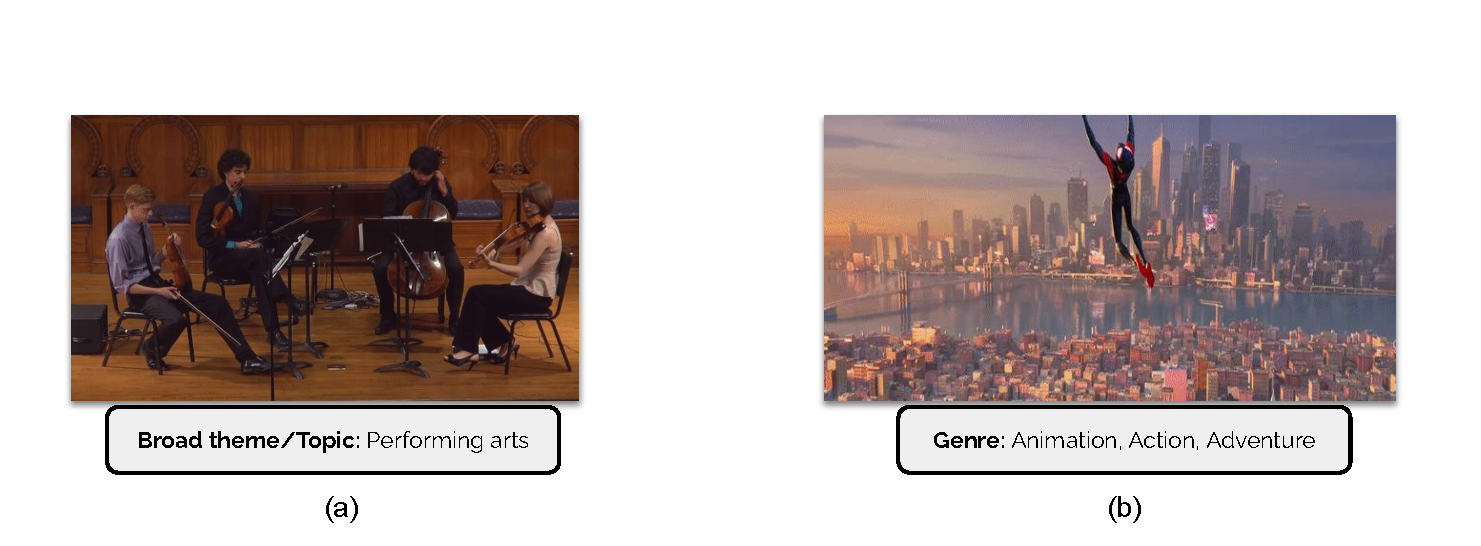
\includegraphics[width=\textwidth]{figures/macro_scale_understanding.pdf}
    \caption{Macro-level understanding examples (a) \textbf{Broad theme/topic:} Performing arts (b) \textbf{Genre:} Animation/action/adventure}
    \label{macro_scale_understanding}
\end{figure}
\subsection{Instance-level content understanding}
Instance level refers to content understanding at the scale of individual entities like objects and persons w.r.t. different attributes like \textbf{appearance}, \textbf{perceived emotional state}, \textbf{gender}, \textbf{age}, \textbf{skintone} and \textbf{occupation}. For example, in Fig \ref{instance_scale_understanding} (a) and (b), the instance-level view refers to the person with the green bounding box and the associated attributes of perceived age, gender, and affective state. In our work, we look at instance-level content understanding in terms of estimating the person's affective state.
\begin{figure}
 \centering
    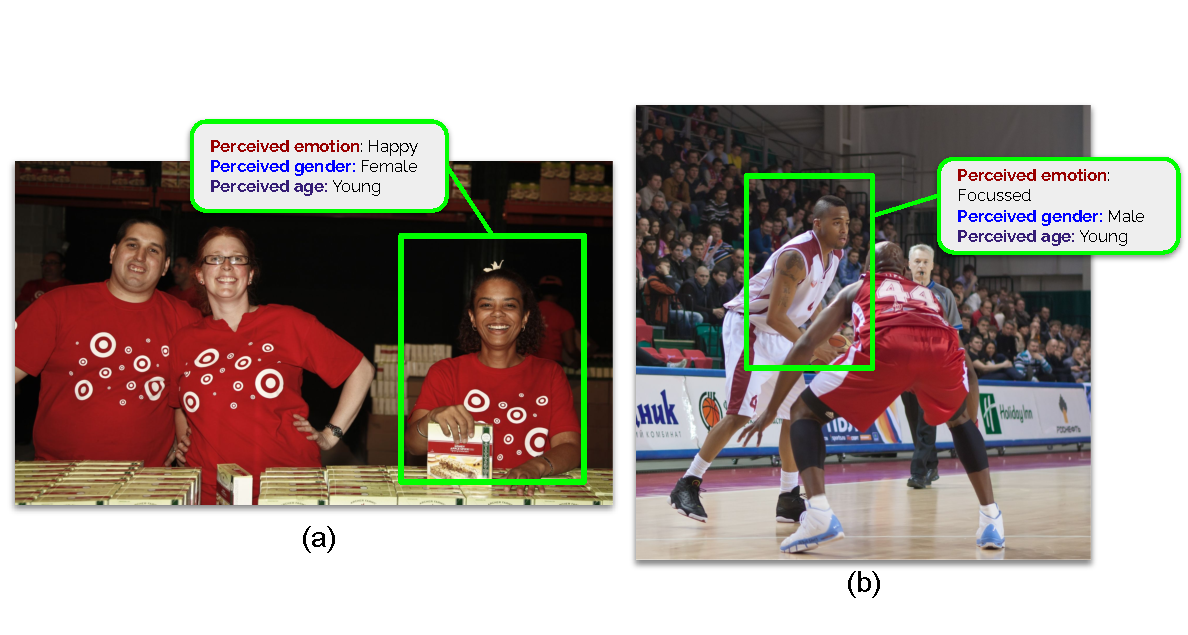
\includegraphics[width=\textwidth]{figures/instance_level_scale_understanding.pdf}
    \caption{Instance-level understanding examples. Image source: \cite{Gustafson2023FACETFI}}
    \label{instance_scale_understanding}
\end{figure}
\section{Organization and contributions}
In this section, we provide the basic outline of the thesis proposal. The proposed thesis statement is given as follows:
\begin{tcolorbox}[width=\textwidth]
Context-guided attention improves multi-modal content understanding at diverse scales.
\end{tcolorbox}
We develop contextual approaches for improved multimodal content understanding at different scales: \textbf{instance-level} and \textbf{macro-level}.  In terms of input sources, we consider multi-modal media content, including \textbf{movies}, \textbf{TV shows}, \textbf{advertisements}, and \textbf{natural scene images}. Looking at the multimodal content from both instance and macro-level viewpoints provides a holistic understanding of given inputs. In terms of the distinction between context and modalities, we use modalities available in input sources to extract diverse forms of contextual information. Further, dissimilar modalities can provide similar types of contextual information. Certain examples of contextual information obtained through multiple modalities are as follows: 

\begin{itemize}
    \item  \textbf{Visual modality:} Captures \textbf{\textit{spatial/temporal}} context through visual semantic units, i.e., objects and persons captured over images and videos.
    \item  \textbf{Language modality:} Captures \textbf{\textit{spatial (semantic)/foreground}} context through foreground based natural language descriptions of images.
    \item  \textbf{Audio modality:} Captures \textbf{\textit{temporal}} context through audio events, background music and speech.
\end{itemize}

\begin{figure}[h!]
    \centering
        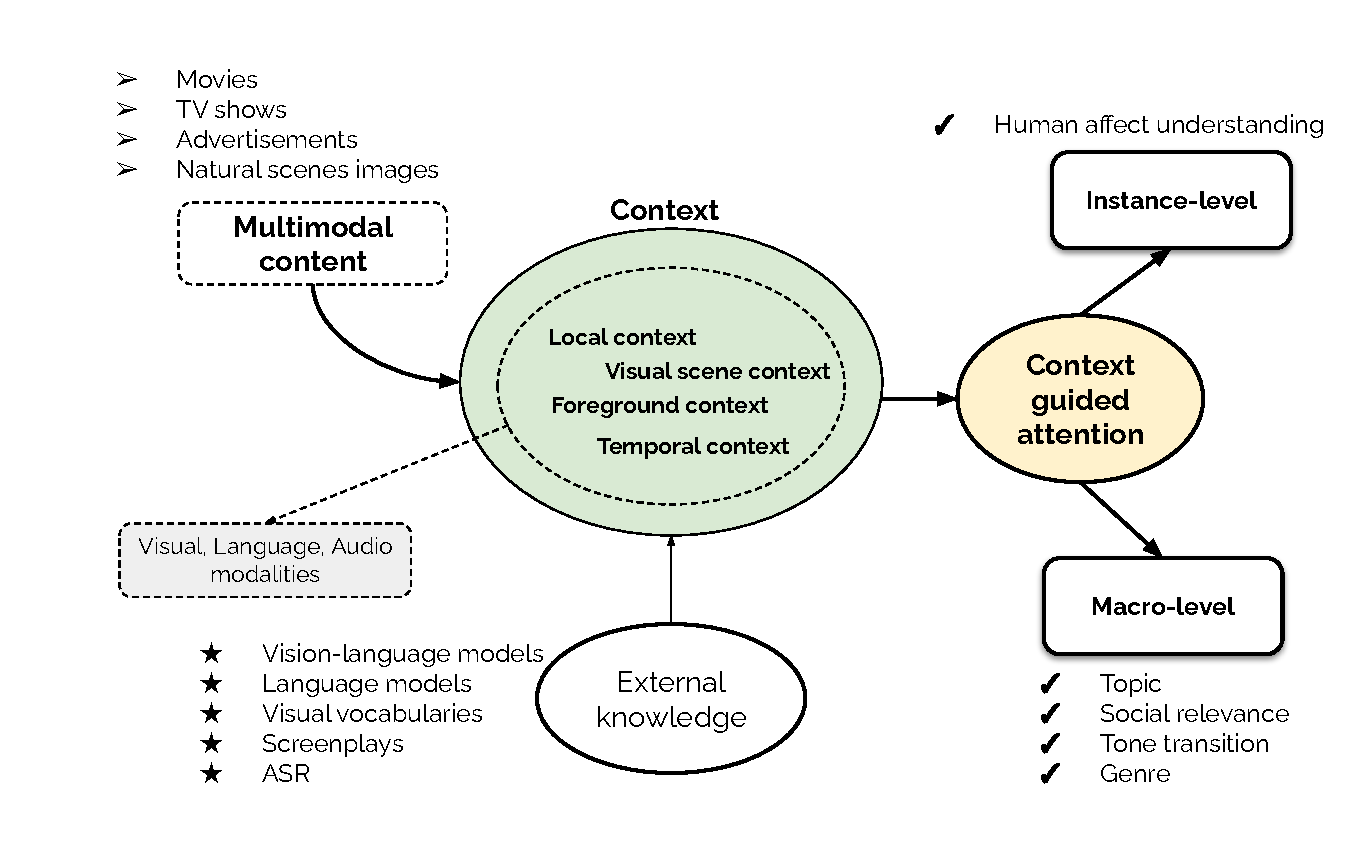
\includegraphics[width=\textwidth]{figures/Overview_diagram.pdf}
        \caption{Organization of the thesis proposal with different components}
        \label{proposalorganization}
\end{figure}

For example, both visual and audio modalities provide the necessary temporal context for various content-understanding tasks.
\par 
In the case of context processing, we leverage external knowledge from pretrained sources like vision-language models, language models, automatic speech recognition models, and domain-specific sources like screenplays and visual vocabularies. 
An outline of the proposal is shown in Fig \ref{proposalorganization}, showing the relationships between input multimodal content and content understanding at different scales. For processing the contextual information, we propose context-guided attention mechanisms to improve multimodal content understanding at two scales: macro-level and instance-level. We consider multi-modal media content, including \textbf{movies}, \textbf{TV shows}, \textbf{advertisements}, and \textbf{in-the-wild} videos as the primary input sources for exploration.
We combine the above-mentioned inputs in a content understanding framework in the following sequence of chapters:

\begin{enumerate}
    \item \textbf{Chapter 2}: We explore the problem of visual scene context processing in multi-modal data esp., movies, by leveraging external knowledge from pretrained multimodal model, i.e., CLIP \cite{Radford2021LearningTV} and domain-specific sources like screenplays, visual vocabularies. Further, we show the utility of visual scene context in improving macro-level content understanding in terms of genre.
    
    \item \textbf{Chapter 3}: We utilize our insights from Chapter 2 to propose a multimodal context fusion approach based on attention mechanism for human affect (\textbf{instance-level}) understanding in natural scenes and TV shows.
    
    \item \textbf{Chapter 4}: We explore the fusion of foreground and temporal context through multiple input modalities for macro-level understanding in advertisement videos along the lines of topic, tone transitions, and social relevance. 
    
    \item \textbf{Chapter 5}: We propose an efficient information-theoretic framework to fuse contextual information in multimodal pretrained transformers for content understanding tasks across different scales.
\end{enumerate}

\textbf{Chapter 5} is an ongoing work and will be extended into post-proposal for integration into the final thesis dissertation.


% Research Topic 1
\include{ResearchTopic1}

% More Research Topics
% \include{ResearchTopic2}

% Conclusion and ongoing work
\chapter{Conclusion and ongoing work}
\label{cha:conclusion}

Here, we would like to revisit the thesis statement before setting directions for ongoing/future work.

\begin{tcolorbox}[width=\textwidth]
Context-guided attention improves multi-modal content understanding at diverse scales.
\end{tcolorbox}


Till now, we have developed models based on context-guided attention for macro/instance level content understanding tasks w.r.t. domains of movies, TV shows, natural scenes, and advertisements. The content understanding tasks are reliant on the representations learned through context-guided attention mechanisms. Here, we would like to pose the following question regarding the enhancement of these learned representations:

\begin{itshape}
Q: Can we guide the representations learned through context-guided attention to be optimal yet robust for the given macro/instance level task?
\label{context:macro instance level}
\end{itshape}

In terms of guidance, we would like to consider the available knowledge from pretrained multimodal models. With the increase in web-based data sources, there is a trend toward the curation of large-scale weakly aligned datasets consisting of images/videos and noisy descriptions like LAION-5B \cite{schuhmann2022laionb}, CC-12M \cite{changpinyo2021cc12m}, WebVid \cite{Bain21}. The curation of these large-scale sources has led to the rise of multimodal pretraining \cite{wang2022MMPTMSurvey}, where transformer-based models are guided by certain objectives as follows:
\begin{itemize}

  \item \textbf{Image-text matching:} Detect whether the image and text pairs are aligned with each other  
 \item \textbf{Word-region alignment:} Detect whether certain words in the descriptions are matched to image regions
 \item \textbf{Caption generation:} Generate a natural language caption to match the given description with the image
 
\end{itemize}

The aforementioned pretraining tasks are certain examples of objectives used for large-scale models and by no means comprise an exhaustive list. The pretraining stage is followed by subsequent finetuning operations for a wide variety of downstream classification and generative tasks, as mentioned below:

\begin{itemize}

    \item \textbf{Classification tasks:} Visual-question answering, Video-language inference, Visual entailment, Category recognition, Multi-modal sentiment analysis
    \item \textbf{Generative tasks:} Image/Video captioning, Visual dialogue, Multimodal machine translation
    
\end{itemize}
 An outline of the pretraining and finetuning operation is shown in Fig \ref{multimodal pretraining}.

 \begin{figure}[h!]
    \centering
    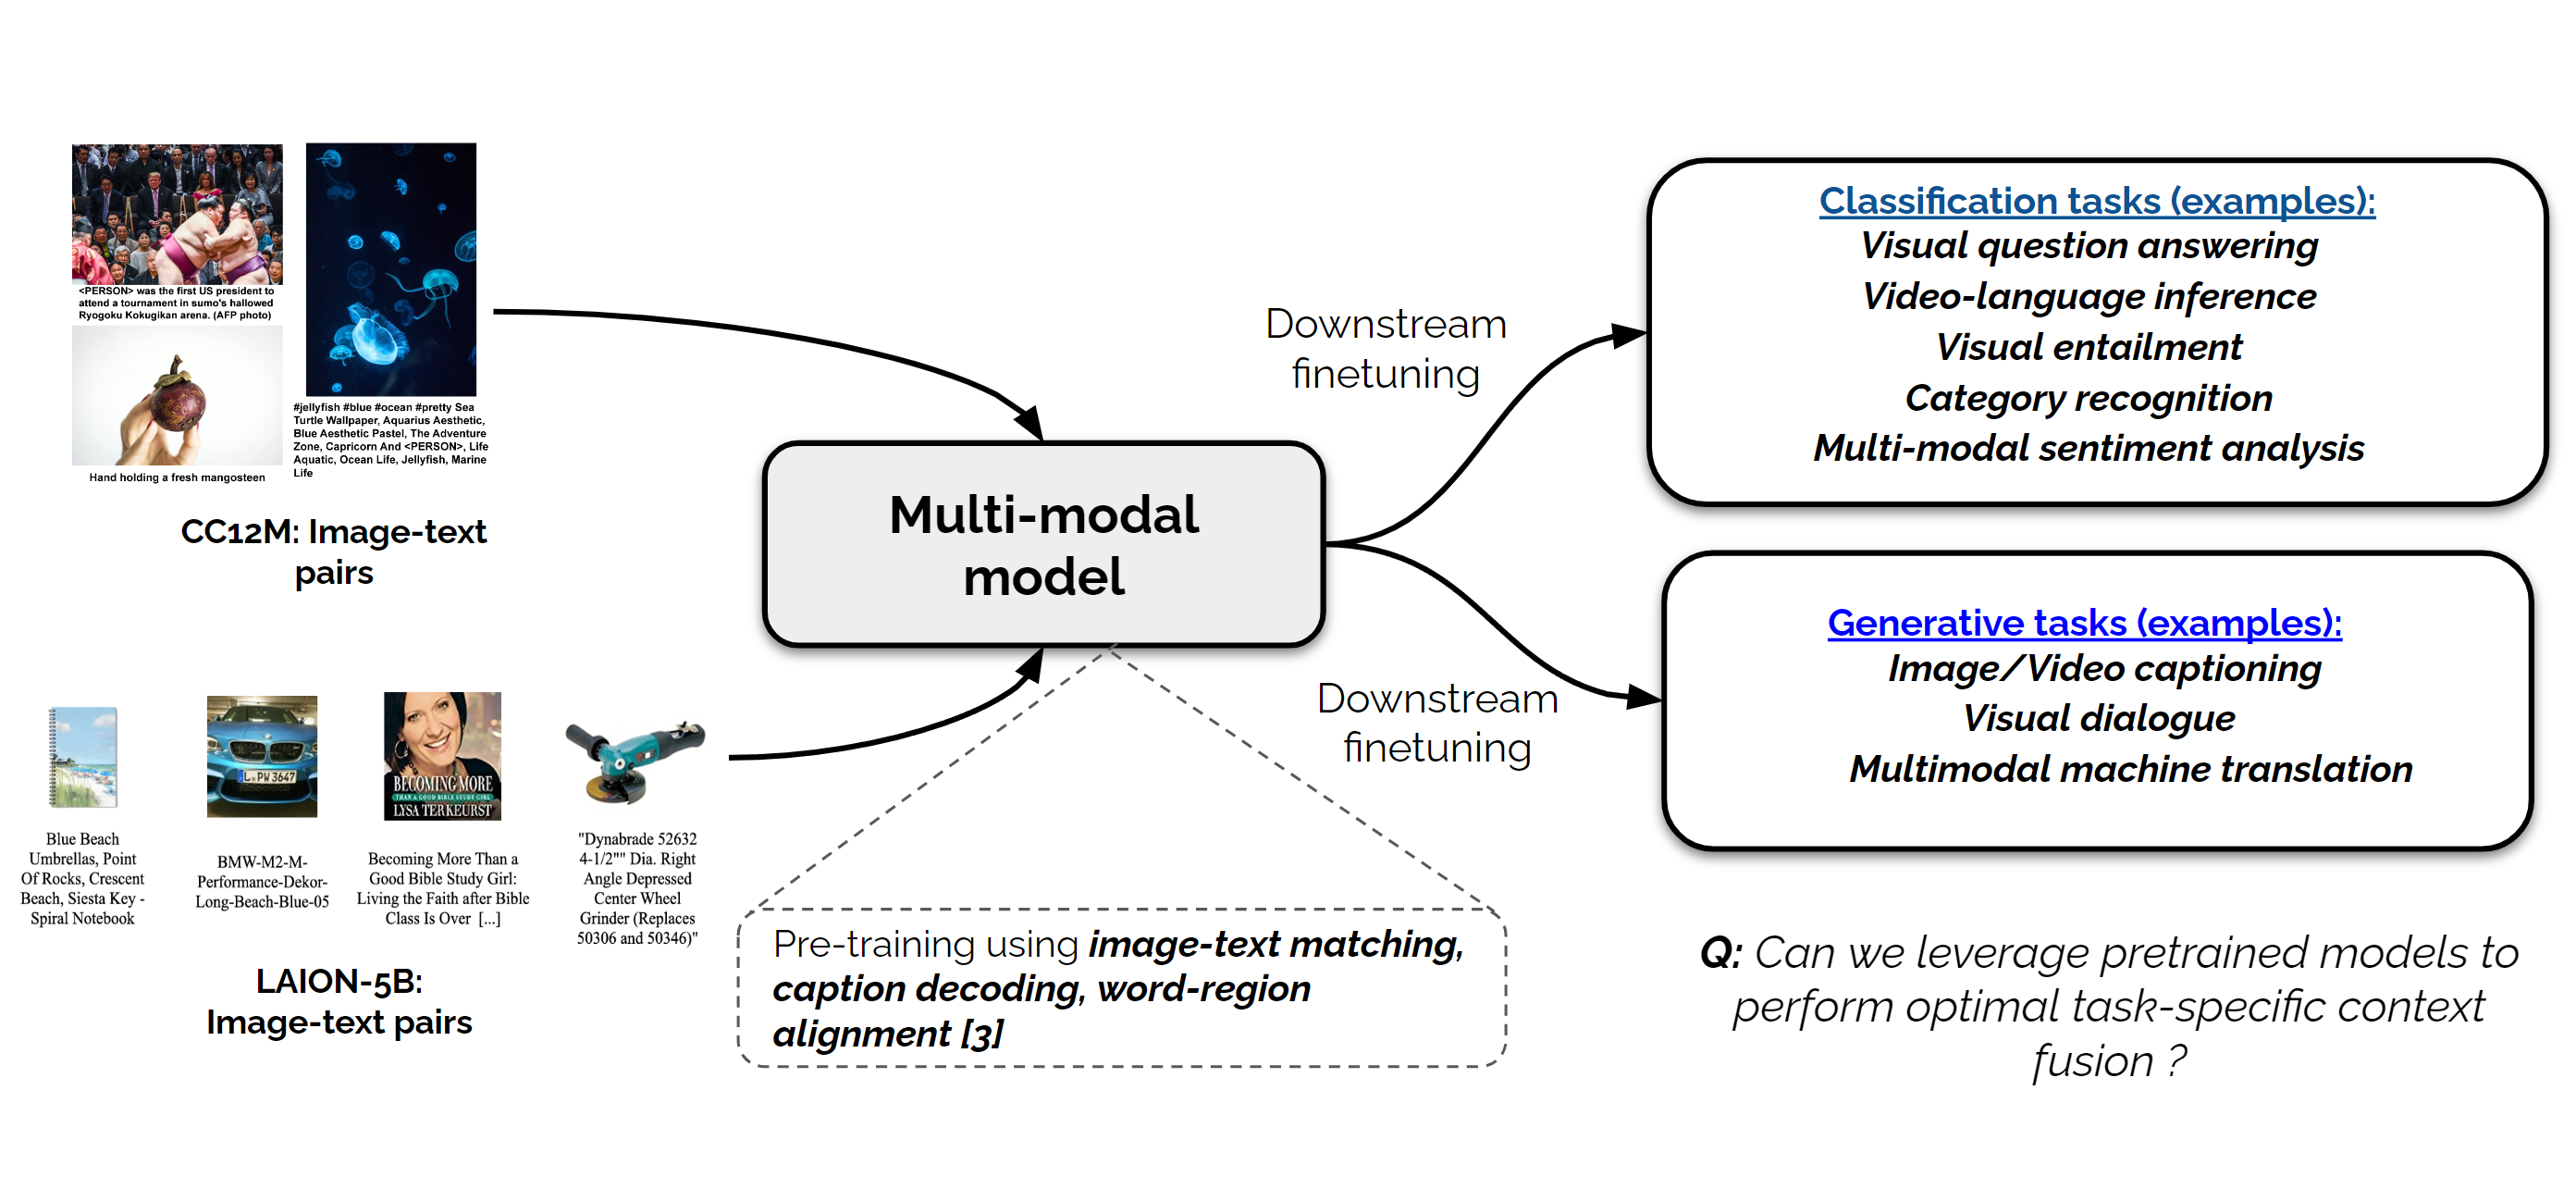
\includegraphics[width=\textwidth]{figures/multimodal_pretraining.png}
    \caption{Pretraining and finetuning operation pipeline in multimodal models.}
    \label{multimodal pretraining}
 \end{figure}

Hence we would like to recast the previous mentioned question to include the role of multimodal pretrained knowledge as follows:

\begin{itshape}
Q: Can we leverage existing large-scale multimodal knowledge to obtain optimal yet robust context-guided representations for given macro/instance-level tasks?
\end{itshape}

With this question, we introduce the concept of Information Bottleneck and how it can be used to obtain optimal yet robust representations for a given task.

\section{Information Bottleneck}

The information bottleneck principle \cite{Tishby2015DeepLA} formulates the goal of deep learning as a trade-off between compression and predictive power. If a given task has associated inputs $X$ and labels $Y$ and the intermediate layer representations of a deep learning model are denoted by $T$, then the optimal task-specific representation can be obtained through the following lagrangian formulation:

\begin{equation}
    L_{IB}= I(Y;T) - \beta I(X;T)
\end{equation}

Here, the objective aims at 
\begin{itemize}
    \item \textbf{Increasing predicting power:} Maximize the mutual information (MI) between labels $Y$ and representations $T$. 
    \item \textbf{Representation compression:} Minimize the mutual information (MI) between inputs $X$ and representations $T$.
\end{itemize}
The parameter $\beta$ controls the relative contributions of the two objective terms. In our case, we would like to explore the usage of information bottleneck as a regularization objective for pretrained multimodal models and its impact on macro and instance-level content understanding tasks under a variety of input settings. We outline our proposed work in the following sections:

\subsection{Related work}
Information Bottleneck (IB) has been utilized for low-resource finetuning of BERT for natural language inference and sentiment analysis tasks in \cite{Mahabadi2021VariationalIB}. Additional usage of information bottleneck includes its usage as task-specific regularizer for learning adversarially robust representations in language models \cite{wang2021infobert}. In the domain of multimodal learning, IB as a regularizer has enabled learning of multimodal representations robust to linguistic variations, image corruptions for visual question answering task \cite{Jiang2022CorrelationIB}. 

\subsection{Information bottleneck and multimodality}

\begin{figure}
     \centering
    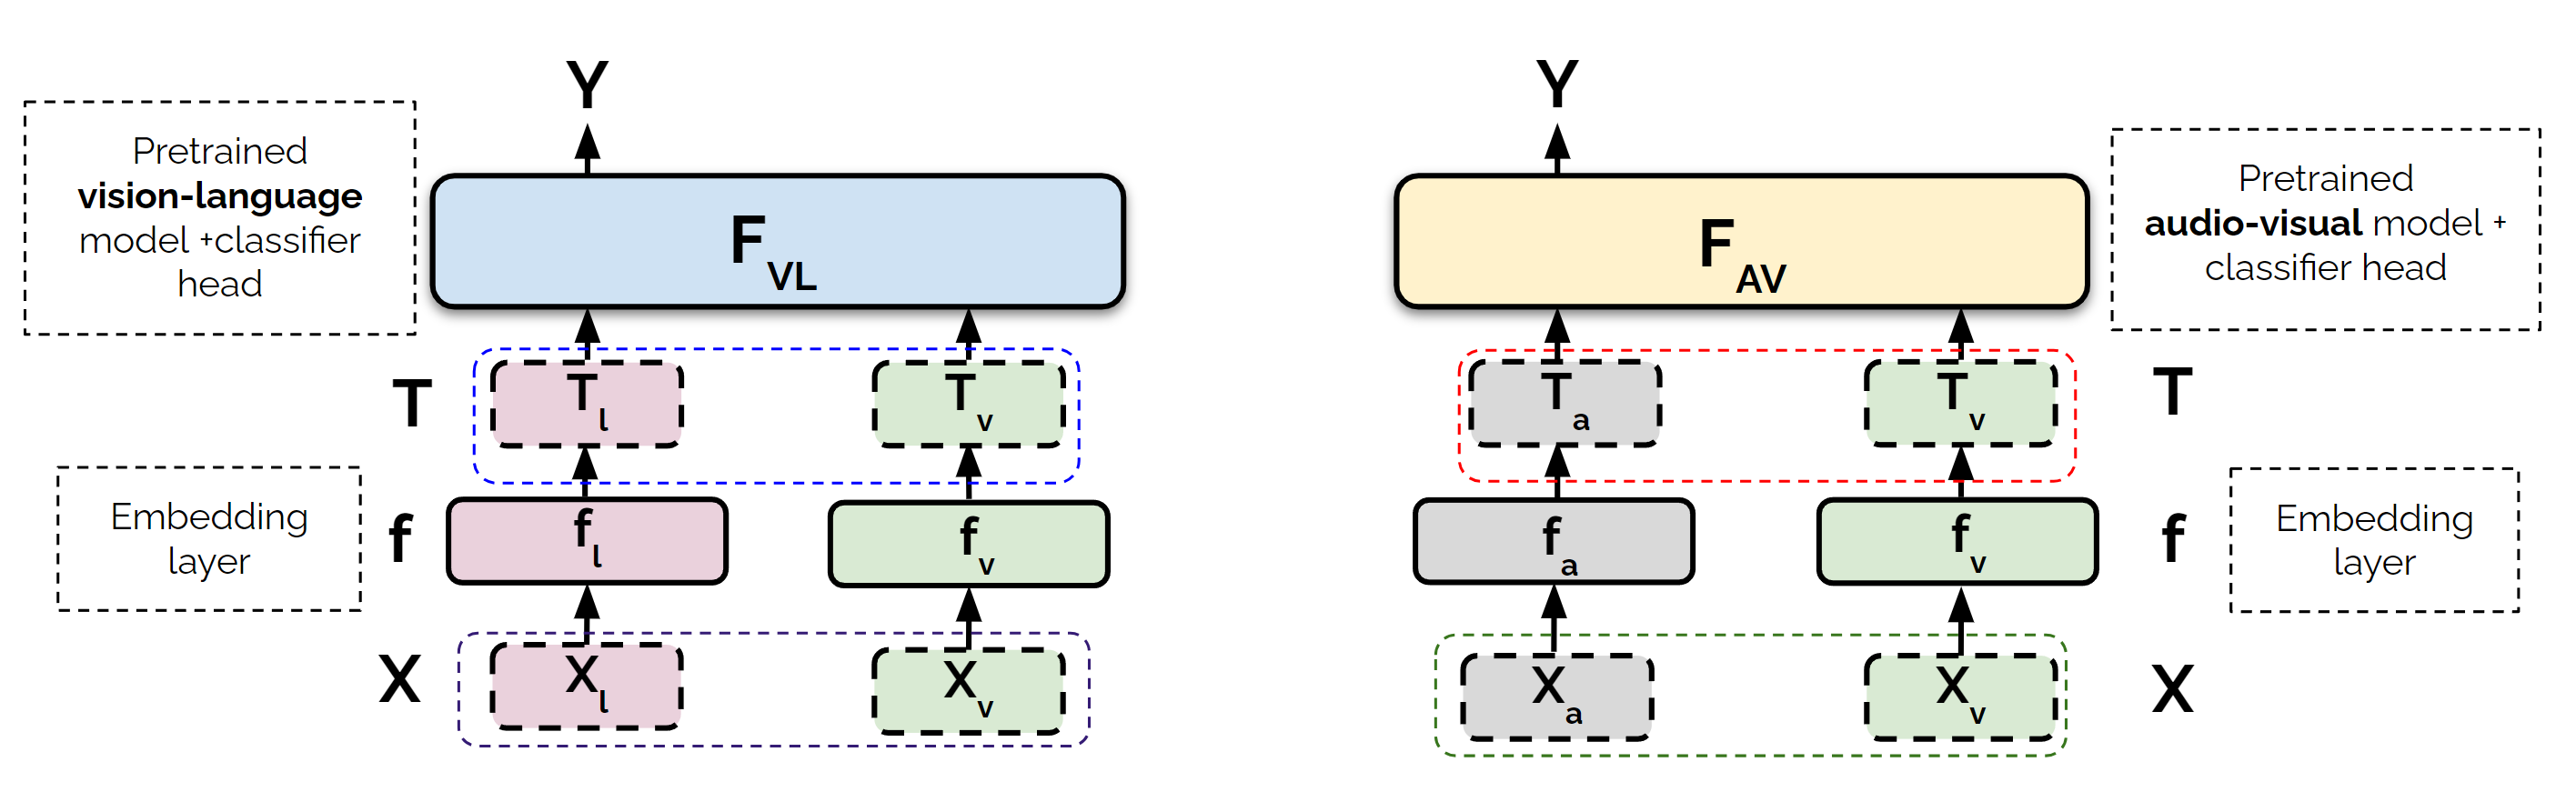
\includegraphics[width=\textwidth]{figures/multimodal_IB.png}
    \caption{Multimodal architecture outline for information bottleneck.}
    \label{multimodal pretraining}
\end{figure}

The base multimodal pretrained architecture to be considered for information bottleneck-related study is shown in Fig \ref{multimodal pretraining} . Given two modalities $m_{1}$ and $m_{2}$, the sequence of operations can be listed as follows:

\begin{align}
    T_{m_{1}}&=f_{m_{1}}(X_{m_{1}}), T_{m_{2}}=f_{m_{2}}(X_{m_{2}})\\
    Y&=F_{m_{1}m_{2}}([T_{m_{1}},T_{m_{2}}])
\end{align}
Here $T_{m_{i}}$ refers to the input embeddings for modality $m_{i}$ and $F_{m_{1}m_{2}}$ refers to the multimodal encoder for predicting the labels. For the multimodal setting, the information bottleneck regularizer can be written as follows:

\begin{equation}
    L_{IB}= I(Y;\{T_{m_{1}},T_{m_{2}}\}) - \beta I(\{X_{m_{1}},X_{m_{2}}\};\{T_{m_{1}},T_{m_{2}}\})
\end{equation}

\subsection{Proposed work (A) - Optimal task-specific representations}
\label{Optimal task-specific representations}
In the first part of the proposed work, we would like to benchmark the performance of various multimodal models under the impact of information bottleneck for content understanding tasks. Since finetuning multimodal models is a memory-intensive operation, we would like to explore the parameter settings under which optimal task-specific representations can be extracted after using the information bottleneck as a regularizer. The outline of the proposed work can be found in Fig \ref{optimal_task_representations}.
The context-processing operation extracts contextual information from the given multimodal content through various modalities. The processed contextual information is passed as input to a pretrained multimodal model with a wide variety of parameter settings:
\begin {itemize}
\item \textbf{Linear-Probe:} Finetuning of the task-specific classifier head only and complete freezing of the multimodal encoder.
\item \textbf{Parameter efficient techniques:} Usage of parameter efficient techniques like LoRA, Adapters, prefix tuning for the multimodal encoder
\item \textbf{Full finetuning:} Complete finetuning of the multimodal encoder.
\end{itemize}
For the above parameter settings, we would like to investigate the impact of information bottleneck guidance while finetuning for a host of macro and instance-level tasks as follows:

\begin{itemize}
    \item \textbf{Advertisement video understanding:} Proposed MM-AU Benchmark
    \item \textbf{Hateful content detection:} Hateful memes \cite{Kiela2020TheHM} dataset
    \item \textbf{Movie understanding:}  Movie genre classification \cite{2019Moviescope}, MMIMDB \cite{Arevalo2017GatedMU}
    \item \textbf {Human affect understanding:} Emotic \cite{kostiPAMI}, CAER \cite{CAER-S}
\end{itemize}
\begin{figure}
 \centering 
 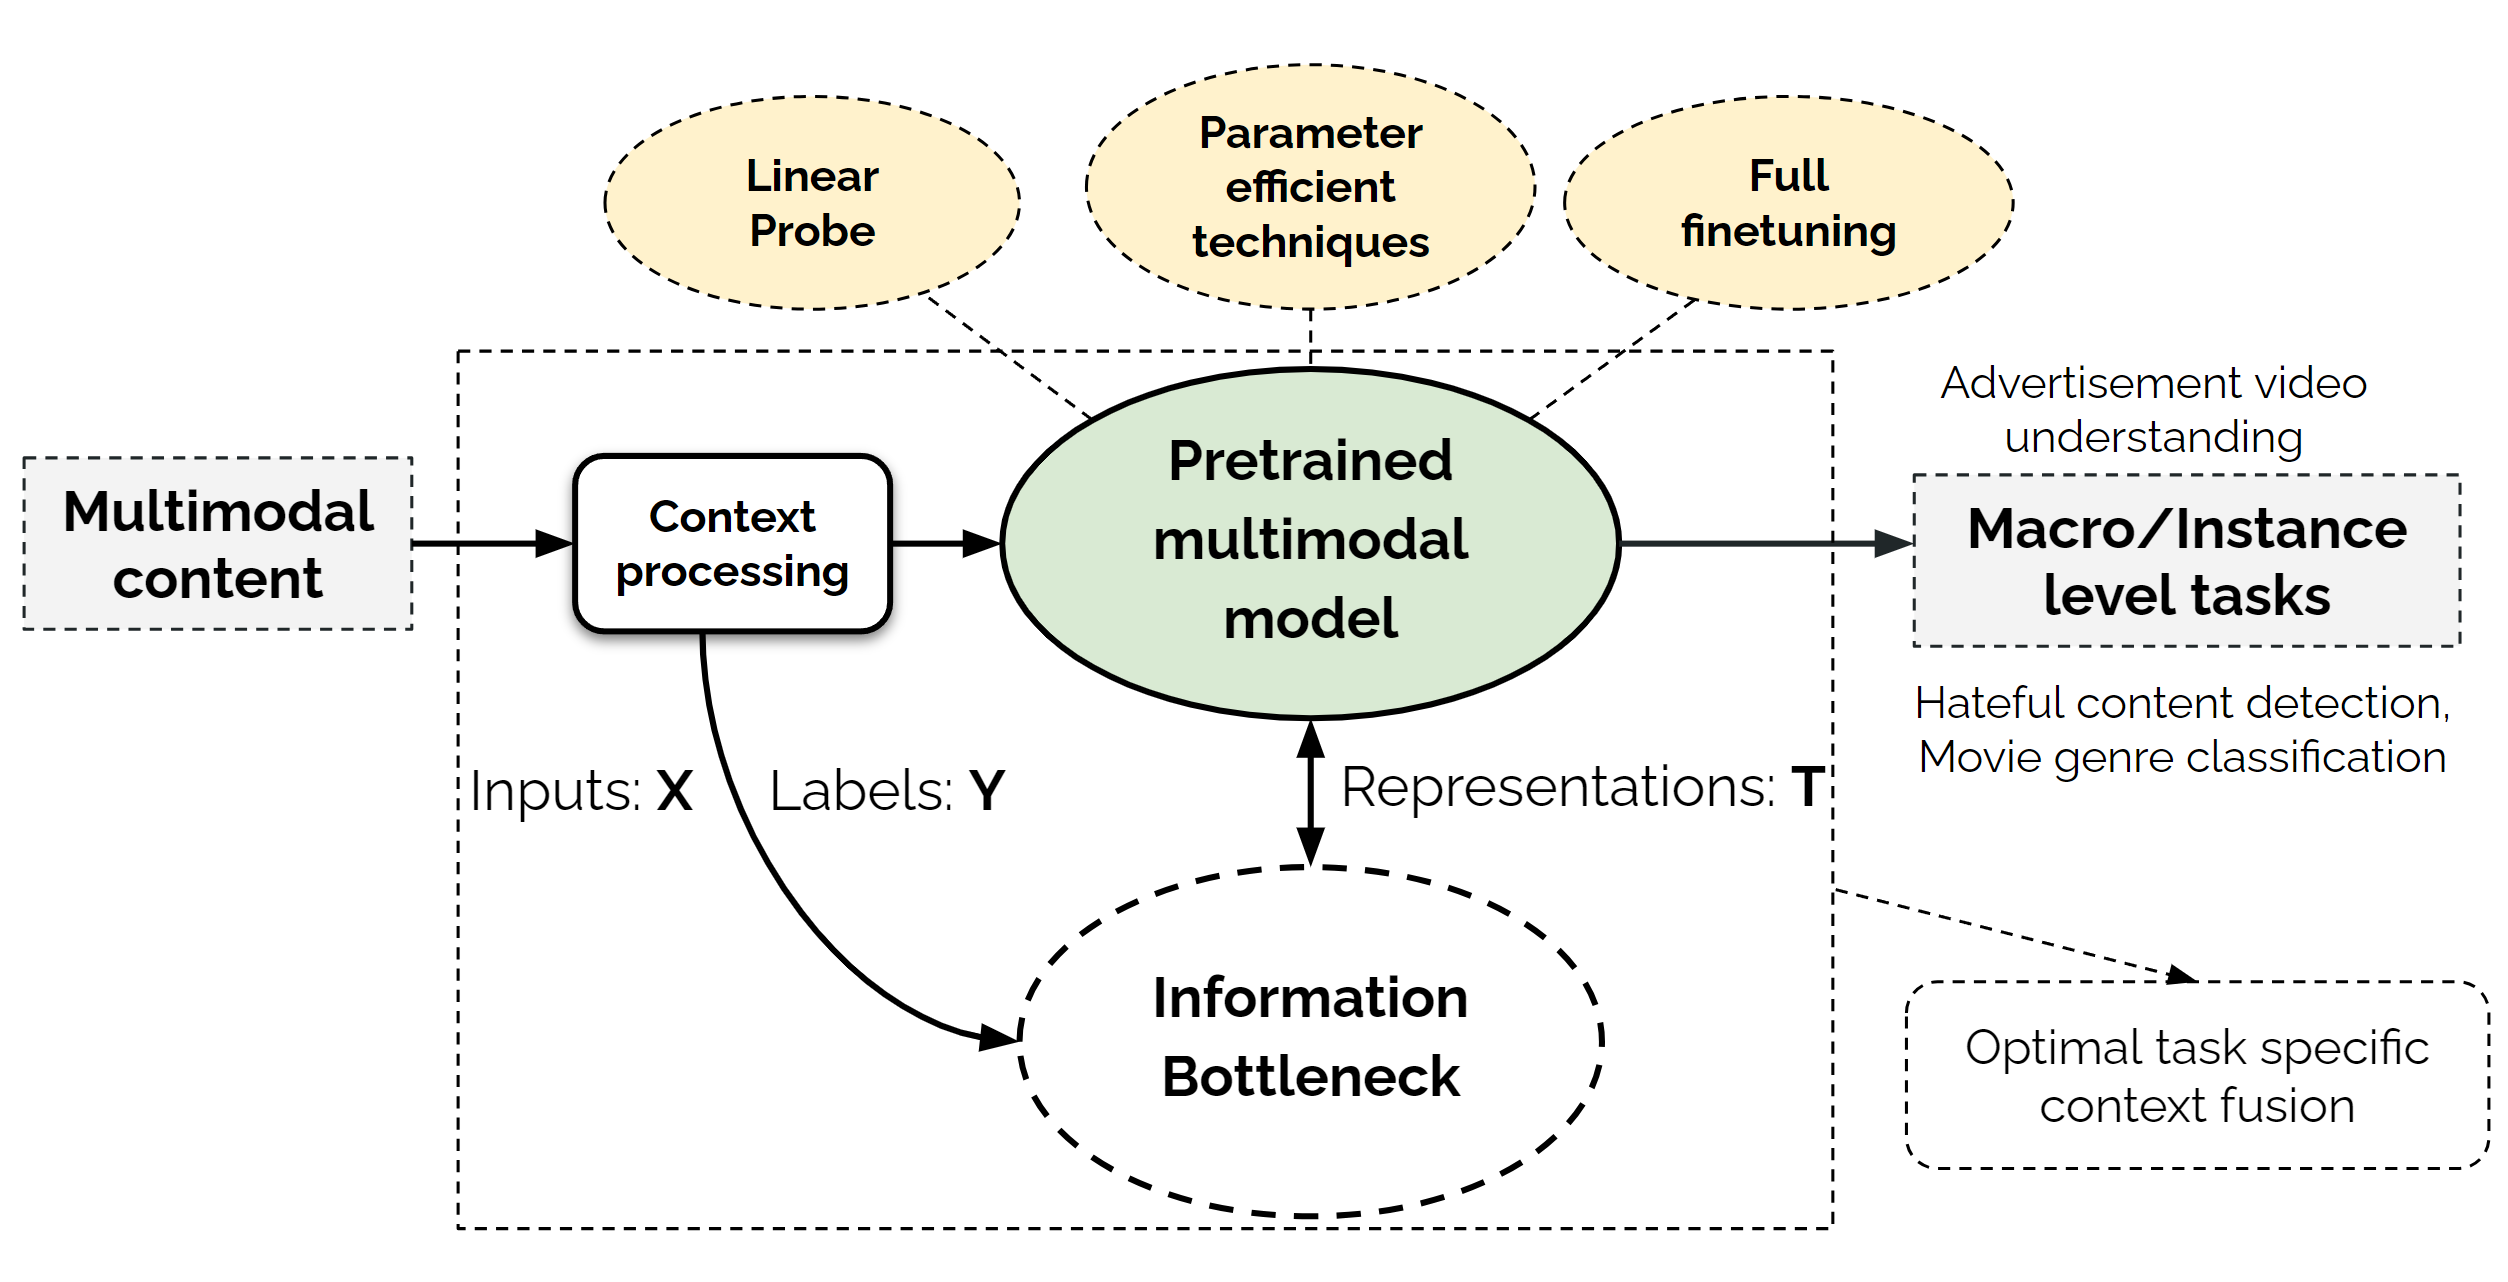
\includegraphics[width=\textwidth]{figures/optimal_task_representations.png}
 \caption{Optimal macro and instance-level task representations based on information bottleneck under different parameter settings}
 \label{optimal_task_representations}
\end{figure}

In terms of architecture, we plan to use the following based on different modality combinations:
\begin{itemize}
\item \textbf{Vision-language:} BLIP-2 \cite{Li2023BLIP2BL}, ViLT \cite{Kim2021ViLTVT}
\item \textbf{Audio-visual:} UAVM model \cite{uavm_gong}
\end{itemize}


\subsection{Proposed work (B) - Characterizing robustness}

Our previous approaches regarding macro and instance level content understanding relied on the assumption that the input sources are free from corruption. However, in real-life settings, the modalities associated with input sources undergo corruption as mentioned in the following examples:

\begin{itemize}
 \item \textbf{Acquisition failure:}  Failure of camera sensors in traffic intersections.
 \item \textbf{Privacy concerns:} Privacy restrictions on accessing social media posts or chats.
 \item \textbf{Noise corruptions:} Excessive noise in audio recordings to be used for emotion classification
\end{itemize}

In the second part of our proposed work, we plan to use the information bottleneck regularizer under the settings of corrupted modalities for pretrained multimodal models. The overall goal is to determine the robustness of the pretrained models with and without information bottleneck regularizer during finetuning. An outline of the corrupted modality setting with our previous optimal task-specific representation framework based on information bottleneck (IB) is shown in Fig \ref{robustness_multimodal_models}.

\begin{figure}
 \centering 
 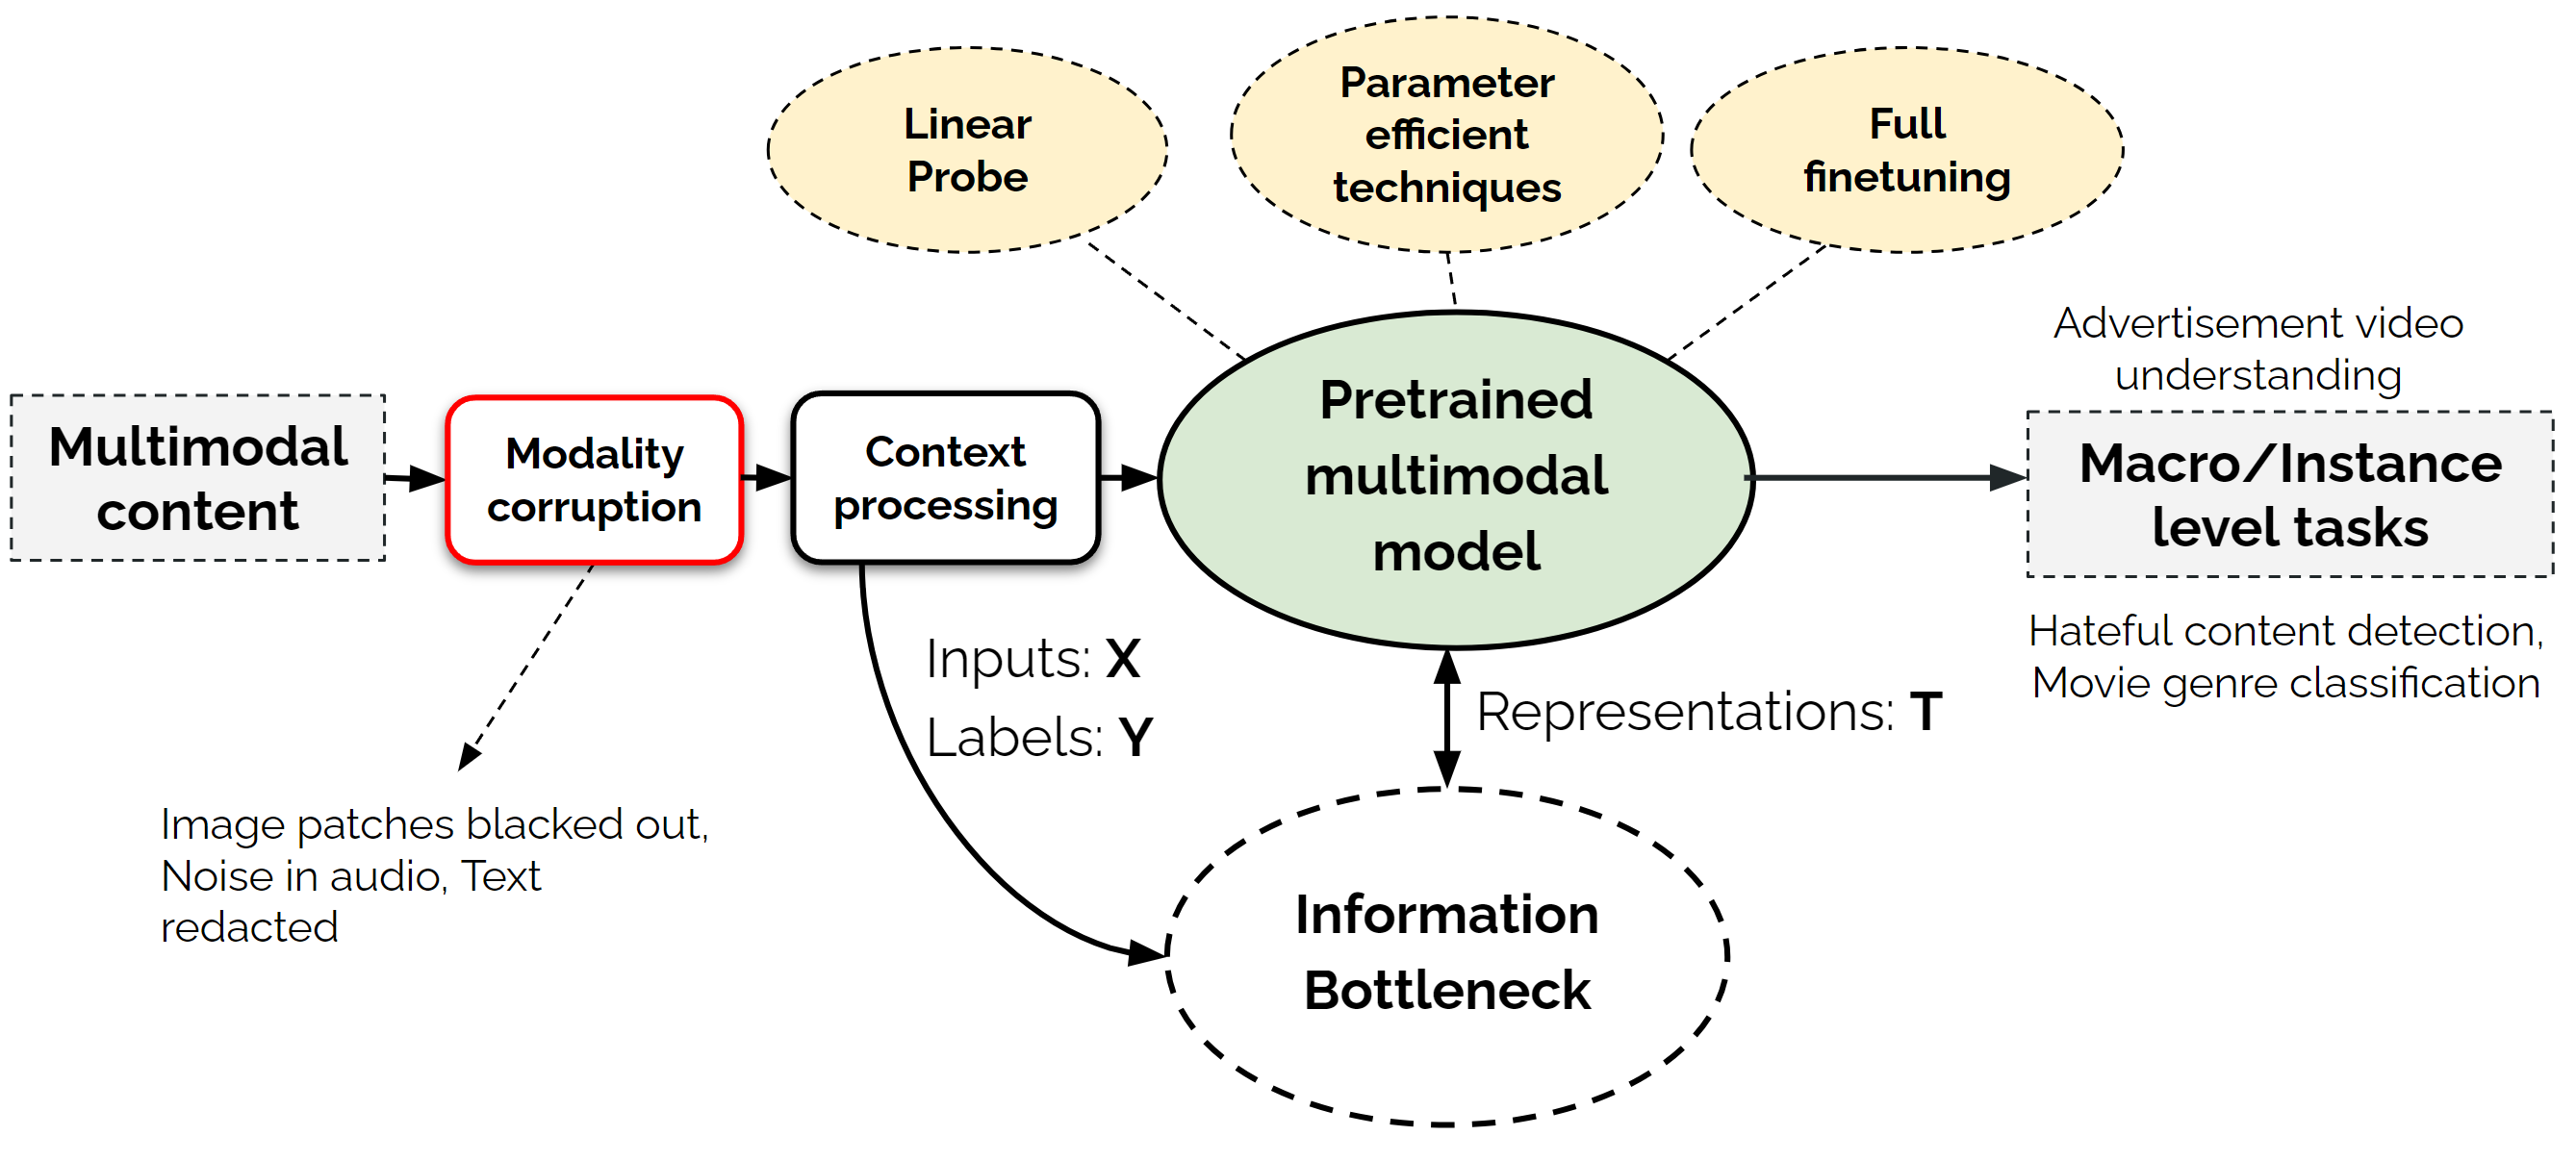
\includegraphics[width=\textwidth]{figures/robustness_multimodal_models.png}
 \caption{Optimal macro and instance-level task representations based on information bottleneck under different parameter settings}
 \label{robustness_multimodal_models}
\end{figure}

We plan to consider the following training and testing scenarios in the robustness study setting:

\begin{itemize}

\item \textbf{Scenario A:} Finetune multimodal model under different parameter settings with IB regularizer and non-corrupted modality inputs.
\item \textbf{Scenario B:} Finetune multimodal model under different parameter settings with IB regularizer and corrupted modality inputs
\item \textbf{Scenario C:} Finetune multimodal model under different parameter settings with IB regularizer and mutual information (MI) maximization between non-corrupted inputs and multimodal representations.

\end{itemize}

In the above-mentioned scenarios, the evaluation will be performed using corrupted modality data. We plan to use the datasets and architectures mentioned in the previous section for this study as well. 


% Using single-space for reference list.
\begin{singlespace}
% Bibliography
\phantomsection
\addcontentsline{toc}{chapter}{References}%
\markboth{References}{References}%
% If you use BibLaTeX
\printbibliography[title=References]
% If you use BibTeX
% \bibliographystyle{plain}
% \bibliography{references}
\end{singlespace}

% Appendices
\phantomsection
\addcontentsline{toc}{chapter}{Appendices}%
\markboth{Appendices}{Appendices}%
\chapter*{Appendices}
\renewcommand\thesection{\Alph{section}}
\renewcommand*{\thesubsection}{\Alph{section}.\arabic{subsection}}
\begingroup
\numberwithin{equation}{section}
% Appendix source files
\section{MovieCLIP dataset}
\label{app:scene_categories}

\subsection{Scene classes distribution wrt sources}
Here \textbf{Movie Slugline} refers to the set of labels obtained exclusively from sluglines in movie scripts. \textbf{Common Label} refers to the set of common labels between taxonomy considered in \textbf{HVU} \cite{diba_large_2020} and \textbf{Movie Slugline}. Here \textbf{HVU} \cite{diba_large_2020} refers to the set of labels obtained exclusively from the taxonomy used for curating \textbf{HVU} \cite{diba_large_2020} dataset. \textbf{Human expert} refers to the set of labels added by the human expert during the taxonomy refinement procedure.

\begin{itemize}
    \item \textbf{Movie Slugline:} \textit{tent}, \textit{computer room}, \textit{truck}, \textit{study},
 \textit{gas station}, \textit{cafe}, \textit{shuttle}, \textit{courthouse}, \textit{elevator}, \textit{tower}, \textit{dorm}, \textit{station}, \textit{club}, \textit{lobby}, \textit{mall}, \textit{salon}, \textit{prison}, \textit{bus}, \textit{stairs}, \textit{theater}, \textit{car}, \textit{booth}, \textit{locker room}, \textit{hangar}, \textit{closet},
 \textit{farmhouse}, \textit{post office}, \textit{townhouse}, \textit{ship}, \textit{loft}, \textit{yard}, \textit{zoo}, \textit{funeral}, \textit{art gallery}, \textit{castle}, \textit{subway}, \textit{lounge}, \textit{train}, \textit{morgue}, \textit{museum}, \textit{wagon}, \textit{manor}, \textit{mansion}, \textit{library}, \textit{pool}, \textit{cellar}, \textit{cab}, \textit{safe house}, \textit{classroom}, \textit{helicopter}, \textit{police station}, \textit{courtroom}, \textit{city hall}, \textit{fire station}, \textit{corridor}, \textit{control room}, \textit{airport}, \textit{cabin}, \textit{war room}, \textit{plane}, \textit{press room}, \textit{cottage}, \textit{residence}, \textit{penthouse}, \textit{inn}, \textit{church}, \textit{suburban}, \textit{interrogation room}, \textit{conference room}

 \item \textbf{Common label:} \textit{tunnel, bakery, shack, building, baseball field, hotel, desert, factory, bathroom, downtown, restaurant, village, playground, boxing ring, gym, bridge, beach, workshop, cave, clinic, arena, garden, stage, office, attic, bowling alley, apartment, deck, cockpit, dining room, basketball court, grove, ballroom, forest, house, barn, alley, park, bay, golf course, chapel, home, parking, bar, kitchen, school, swamp, basement, walkway, bedroom, garage, lake, bank, living room, room,
 auditorium, street, valley, casino, hall, waterfall, warehouse,
 tennis court, farm, hospital, palace, estate, river}
 
 \item \textbf{HVU:} \textit{archaeological site, shore,
 batting cage, animal shelter, plaza, hot spring,
 harbor, bullring, sandbank, town, mountain,
 retail, courtyard, sea, road, shooting range,
 pond, stadium, foundry, skyline, amusement park,
 market, laboratory, race track, kindergarten, ice rink}

\item \textbf{Human expert:} \textit{agriculture field, makeup studio, grassland, construction site,
 graveyard, automotive repair, overpass, studio, boat, fair, balcony, battlefield, banquet, phone booth,
 concert hall, meadow}
\end{itemize}

\section{MM-AU Benchmark}
\label{app:topic_categories}
\subsection{Topic categories}

We provide the mapping between Cannes(CC) \cite{cannes-lions}, Ads of the World (AOW)\footnote{https://www.adsoftheworld.com/} and Video-Ads (VA) \cite{Hussain2017AutomaticUO} coding schemes for obtaining the final set of topic categories as follows:

\begin{itemize}
    \item \textbf{Games:} Games and toys [\textcolor{blue}{\textbf{VA}}]; Gaming [\textcolor{red}{\textbf{AOW}}]
    \item \textbf{Household:} Household: Home Appliances, Furnishing [\textcolor{purple}{\textbf{CC}}]; Cleaning products, Home improvements and repairs, Home appliances [\textcolor{blue}{\textbf{VA}}]
    \item \textbf{Services:} Other services i.e. dating, tax, legal, loan, religious, printing, catering, etc. [\textcolor{blue}{\textbf{VA}}]; Professional Services [\textcolor{red}{\textbf{AOW}}].
    \item \textbf{Misc:} Miscellaneous, Business equipment and services [\textcolor{purple}{\textbf{CC}}]; Petfood, Political candidates (Politics) [\textcolor{blue}{\textbf{VA}}]; Pets [\textcolor{red}{\textbf{AOW}}]
    \item \textbf{Sports:} Sports equipment and activities [\textcolor{blue}{\textbf{VA}}]; Sports [\textcolor{red}{\textbf{AOW}}]
    \item \textbf{Banking:} Banking and services [\textcolor{purple}{\textbf{CC}}]; Financial services [\textcolor{blue}{\textbf{VA}}]; Finance [\textcolor{red}{\textbf{AOW}}]
    \item \textbf{Clothing:} Clothing, Footwear \& Accessories [\textcolor{purple}{\textbf{CC}}]; Clothing and accessories [\textcolor{blue}{\textbf{VA}}]; Personal Accessories [\textcolor{red}{\textbf{AOW}}] 
    \item \textbf{Industrial and agriculture:} Industrial, Agriculture Public Interest, Agriculture Professional Services [\textcolor{red}{\textbf{AOW}}]
    \item \textbf{Leisure:} Entertainment \& Leisure [\textcolor{purple}{\textbf{CC}}]; Gambling (lotteries, casinos, etc.) [\textcolor{blue}{\textbf{VA}}]; Recreation, Gambling [\textcolor{red}{\textbf{AOW}}]
    \item \textbf{Publications \& media:} Media \& Publications  [\textcolor{purple}{\textbf{CC}}]; Media and arts [\textcolor{blue}{\textbf{VA}}]; TV Promos, Music, Media, Movies [\textcolor{red}{\textbf{AOW}}]
    \item \textbf{Health:} Healthcare \& Pharmacy [\textcolor{purple}{\textbf{CC}}]; Health care and medications [\textcolor{blue}{\textbf{VA}}]; Health, Pharmaceutical [\textcolor{red}{\textbf{AOW}}]
    \item \textbf{Car:} Cars \& Automotive Products \& Services [\textcolor{purple}{\textbf{CC}}]; Car [\textcolor{blue}{\textbf{VA}}]; Automotive [\textcolor{red}{\textbf{AOW}}]
    \item \textbf{Electronics:} Home electronics and audio-visual [\textcolor{purple}{\textbf{CC}}]; Electronics, Phone, TV and internet service providers [\textcolor{blue}{\textbf{VA}}]; Electronics [\textcolor{red}{\textbf{AOW}}]
    \item \textbf{Cosmetics:} Cosmetics \& Toiletries [\textcolor{purple}{\textbf{CC}}]; Beauty products and cosmetics, Baby products [\textcolor{blue}{\textbf{VA}}]; Beauty [\textcolor{red}{\textbf{AOW}}]
    \item \textbf{Food and drink:} Savoury Foods, Sweet Foods \& Snacks, Non Alcoholic drinks, Alcoholic drinks [\textcolor{purple}{\textbf{CC}}]; Chocolate, Chips, Seasoning, Coffee, Soda, juice, milk, energy drinks, water, Alcohol [\textcolor{blue}{\textbf{VA}}]; Food, Non-Alcoholic Drinks, Confectionery, Alcoholic drinks [\textcolor{red}{\textbf{AOW}}]
    \item \textbf{Awareness:} Charities and non-profit [\textcolor{purple}{\textbf{CC}}]; Environment, Animal rights, Human rights, Safety, Smoking, Alcohol Abuse, Domestic Violence, Self-esteem, cyberbullying [\textcolor{blue}{\textbf{VA}}]; Education, Agency Self-Promo [\textcolor{red}{\textbf{AOW}}]
    \item \textbf{Travel and transport:} Travel \& Transport [\textcolor{purple}{\textbf{CC}}]; Vacation and travel [\textcolor{blue}{\textbf{VA}}]; Transport, Hospitality [\textcolor{red}{\textbf{AOW}}]
    \item \textbf{Retail:} Retail \& e-commerce [\textcolor{purple}{\textbf{CC}}]; Shopping (department stores, drug stores, groceries, etc.) [\textcolor{blue}{\textbf{VA}}]; Retail Services [\textcolor{red}{\textbf{AOW}}]
\end{itemize}
The taxonomy sources are listed within [.] for respective subcategories for the final list of topic categories. 


\section{MM-AU Experiments}
\label{app:language_baselines}
\subsection{Language based reasoning}

We investigate the zero-shot performance of several large language models i.e. \texttt{GPT-4}\cite{OpenAI2023GPT4TR}, \texttt{Opt-IML} \cite{Iyer2022OPTIMLSL}, \texttt{Flan-T5} (XXL,XL,L) \cite{Chung2022ScalingIL} and \texttt{Alpaca} \cite{alpaca} on the benchmark tasks associated with \textbf{MM-AU} dataset. For zero-shot evaluation, we report the results on 1670 non-empty transcripts out of the test split of 1692 samples.
\subsubsection{Flan-T5:}
For \texttt{Flan-T5}, we use the following prompts for the social message (\textbf{SM}), tone transition (\textbf{TT}), topic categorization(\textbf{Topic}) tasks: 
\begin{itemize}

\item \textbf{\underline{TT:}} 
\texttt{<Text from transcript>} \\
\textit{Based on the given text transcript from the advertisement, determine if the advertisement has any transitions in tones.} \\ 
\textbf{OPTIONS:}
\begin{itemize}
\item[-] Transition
\item[-] No transition
\end{itemize}
\textbf{ANSWER:}

\item \textbf{\underline{SM:}}
\texttt{<Text from transcript>} \\
\textit{An advertisement video has a social message if it provides awareness about any social issue. Examples of social issues: gender equality, drug abuse, police brutality, workplace harassment, domestic violence, child labor, environmental damage, homelessness, hate crimes, racial inequality etc. Based on the given text transcript, determine if the advertisement has any social message.}\\
\textbf{OPTIONS:}
\begin{itemize}
\item[-] Yes
\item[-] No
\end{itemize}
ANSWER: 

\item \textbf{\underline{Topic:}}
\texttt{<Text from transcript>} \\
\textit{Associate a single topic label with the transcript from the given set:} \\
\textbf{OPTIONS:}
\begin{itemize}
\item [-] Games
\item [-] Household
\item [-] Services
\item [-] Sports 
\item [-] Banking 
\item [-] Clothing 
\item [-] Industrial and agriculture 
\item [-] Leisure 
\item [-] Publications media 
\item [-] Health 
\item [-] Car 
\item [-] Electronics 
\item [-] Cosmetics 
\item [-] Food and drink 
\item [-] Awareness 
\item [-] Travel and transport 
\item [-] Retail 
\end{itemize}
\textbf{ANSWER:}
\end{itemize}

\subsubsection{OPT:} For \texttt{OPT}, we use the following prompt templates for different tasks:

\begin{itemize}

    \item \textbf{\underline{TT:}} \textit{Instruction: In this task, you are given a transcription of an advertisement, determine if the advertisement has any transitions in tones.} \\
    \textbf{Transcription:} \texttt{<Text from transcript>}\\
    \textbf{OPTIONS:}
    \begin{itemize}
    \item[-] Transition
    \item[-] No transition
    \end{itemize}
   \textbf{Answer:}

    \item \textbf{\underline{SM:}} \textit{In this task, you are given a transcription of an advertisement. An advertisement video has a social message if it provides awareness about any social issue. Example of social issues: gender equality, drug abuse, police brutality, workplace harassment, domestic violence, child labor, environmental damage, homelessness, hate crimes, racial inequality etc. Your task is to give label "Yes" if the advertisement given has any social message, otherwise give label "No".} \\
    \textbf{Transcription:} \texttt{<Text from transcript>}\\
    \textbf{Answer:}
    
    \item \textbf{\underline{Topic:}} \textit{In this task, you are given a transcription of an advertisement. Your task is to associate a single topic label with the transcript from the given set.} \\
    \textbf{Transcription:} \texttt{<Text from transcript>}\\
    \textbf{OPTIONS:}
    \begin{itemize}
    \item [-] Games
    \item [-] Household
    \item [-] Services
    \item [-] Sports 
    \item [-] Banking 
    \item [-] Clothing 
    \item [-] Industrial and agriculture 
    \item [-] Leisure 
    \item [-] Publications media 
    \item [-] Health 
    \item [-] Car 
    \item [-] Electronics 
    \item [-] Cosmetics 
    \item [-] Food and drink 
    \item [-] Awareness 
    \item [-] Travel and transport 
    \item [-] Retail 
    \end{itemize}
    \textbf{Answer:}
\end{itemize}

\subsubsection{alpaca:} 
For \texttt{alpaca}, we use the following prompt templates for different tasks:

\begin{itemize}
    \item \textbf{\underline{TT:}} \textit{Instruction: In this task, you are given a transcription of an advertisement determine if the advertisement has any transitions in tones.}\\
\textbf{Transcription}: \texttt{<Text from transcript>}\\
\textbf{Options:}
\begin{itemize}
\item[-] Transition
\item[-] No transition
\end{itemize}
\textbf{Answer:}
\item \textbf{\underline{SM:}} \textit{Instruction: In this task, you are given a transcription of an advertisement. An advertisement video has a social message if it provides awareness about any social issue. Example of social issues: gender equality, drug abuse, police brutality, workplace harassment, domestic violence, child labor, environmental damage, homelessness, hate crimes, racial inequality etc. Based on the given text transcript, determine if the advertisement has any social message. }\\
    \textbf{Transcription:} \texttt{<Text from transcript>}\\
\textbf{Options:}
\begin{itemize}
\item[-] Yes
\item[-] No
\end{itemize}
\textbf{Answer:}
\item \textbf{\underline{Topic:}} \textit{Instruction: In this task, you are given a transcription of an advertisement. Your task is to associate a single topic label with the transcript from the given set.}\\
\textbf{Transcription:} \texttt{<Text from transcript>}\\
\textbf{Options:}
    \begin{itemize}
    \item [-] Games
    \item [-] Household
    \item [-] Services
    \item [-] Sports 
    \item [-] Banking 
    \item [-] Clothing 
    \item [-] Industrial and agriculture 
    \item [-] Leisure 
    \item [-] Publications media 
    \item [-] Health 
    \item [-] Car 
    \item [-] Electronics 
    \item [-] Cosmetics 
    \item [-] Food and drink 
    \item [-] Awareness 
    \item [-] Travel and transport 
    \item [-] Retail 
\end{itemize}
\textbf{Answer:}
\end{itemize}
For \texttt{GPT-4} we use the recently released API to pass the prompts for individual tasks.
For \texttt{Flan-T5} and \texttt{Opt-IML}, we use the publicly available models as a part of Huggingface \cite{wolf-etal-2020-transformers} library. For \texttt{alpaca}, we use the publicly available implementation in Github \cite{alpaca}. The large language models sometimes assign a label to the prediction that does not lie within the set of valid labels for the respective tasks. In the case of those samples, we randomly assign a label from the task-specific label taxonomy. 

\endgroup

% In case your dissertation has multiple volumes.
% \addvolumecontents{thesis_part2}
% \addvolumecontents{thesis_part3}
% \addvolumecontents[lof]{thesis_part2}

\end{document}
